\subsection{Flat plate}
The turbulent flow over a flat plate is investigated. All grids and results are available in~\cite{tmr} under the name: ``2D Zero pressure gradient flat plate''. The problem domain and flow conditions are shown in~\Cref{fig:flat}. The Turbulence Modeling Resource provides five grids, each finer than the next, in order to compare so-called mesh independent results and to perform a grid study. The goal of a grid study is to establish that the obtained results will not vary significantly by further refining the mesh.
\begin{figure}
    \centering
    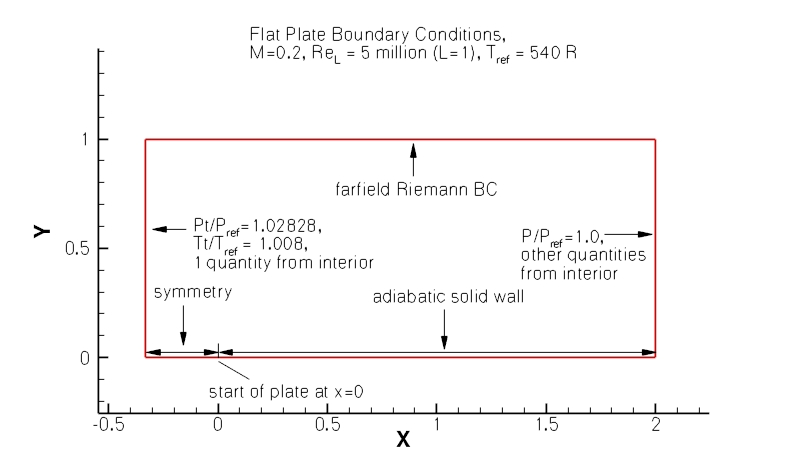
\includegraphics[width=0.7\textwidth]{figs/flat/flatplate.png}
    \caption{Turbulent flat plate case~\cite{tmr}.}
    \label{fig:flat}
\end{figure}
The skin friction coefficient $C_f$ at $x = 0.97$ and drag coefficient $C_D$ are compared to CFL3D, a cell-centered finite volume code developed by NASA, in~\Cref{tab:flat}. They are calculated as:
\begin{align*}
    C_f = \frac{2\tau_w}{\rho_\infty U_\infty^2}\\
    C_D = \frac{2D}{\rho_\infty U_\infty^2 A}
\end{align*}
where $D$ is the drag force and $A$ is the reference area. For this case, the reference area is the length of the plate times its width, i.e. the length of the mesh in the $z$ direction. \Cref{tab:flat} tabulates skin friction coefficient and drag coefficient values.
\begin{table}
\centering
\caption{Flat Plate (Syn3D): Comparison of force coefficients on the finest grid.}
\label{tab:flat}
\begin{tabular}{@{}lcc@{}}
    \toprule
    Solver & $C_D$ & $C_f$ at $x=0.97$ \\
    \midrule
    CFL3D & 0.00286 & 0.00270 \\
    Syn3D & 0.00280 & 0.00269\\
    \bottomrule
\end{tabular}
\end{table}
\Cref{fig:synflatcnvstudy} shows the residual convergence of the density residual and turbulence residual for all grids. The density residual, which is the residual of the mass equation, was driven down to around $10^-4$ on all meshes, which is enough for the sake of this comparison -- differences in the obtained solution field were found to be marginal beyond that point.
\begin{figure}[ht!]
\centering
\begin{subfigure}{.45\textwidth}
  \centering
  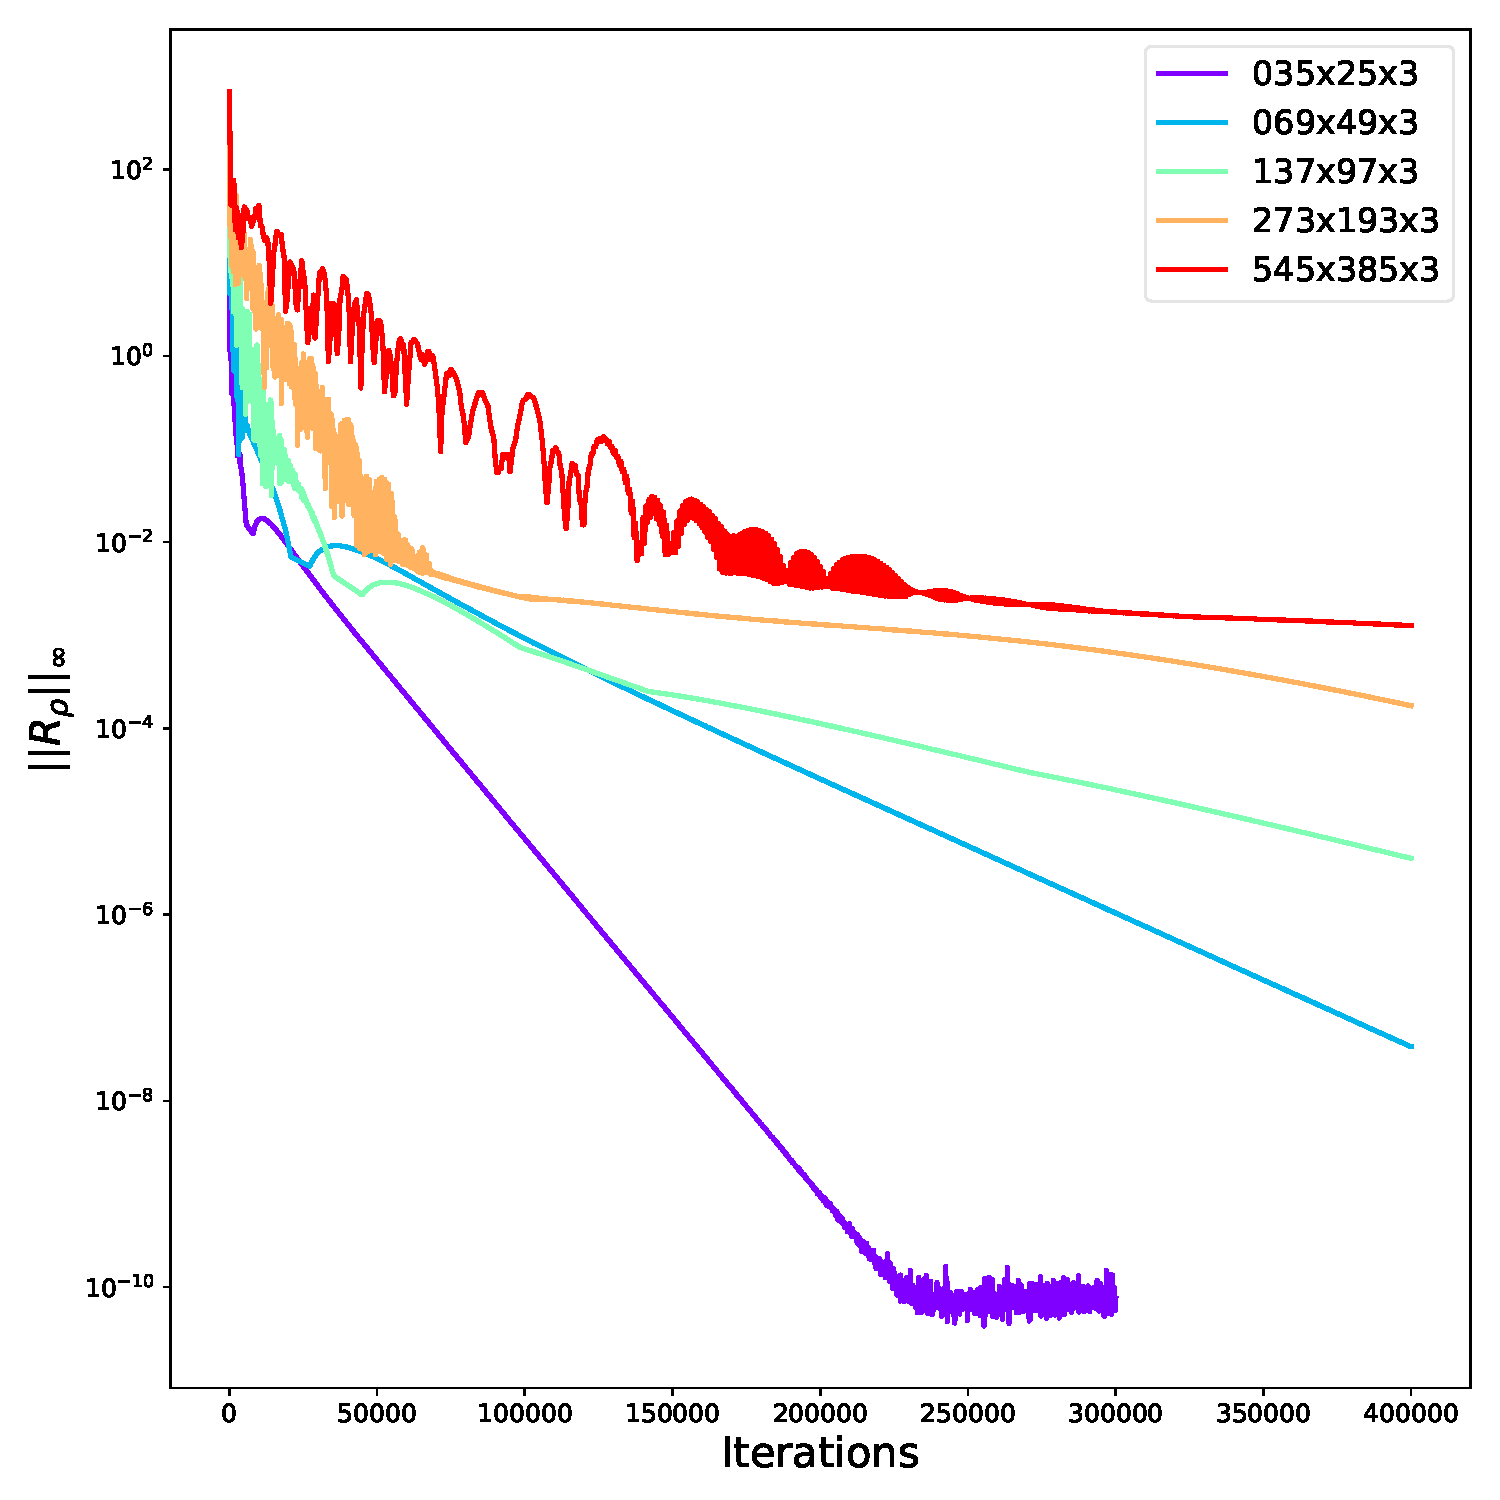
\includegraphics[width=1.0\textwidth]{figs/flat/gov_convergence_gridstudy.pdf}
  \caption{Maximum density residual.}
\end{subfigure}%
\begin{subfigure}{.45\textwidth}
    \centering
    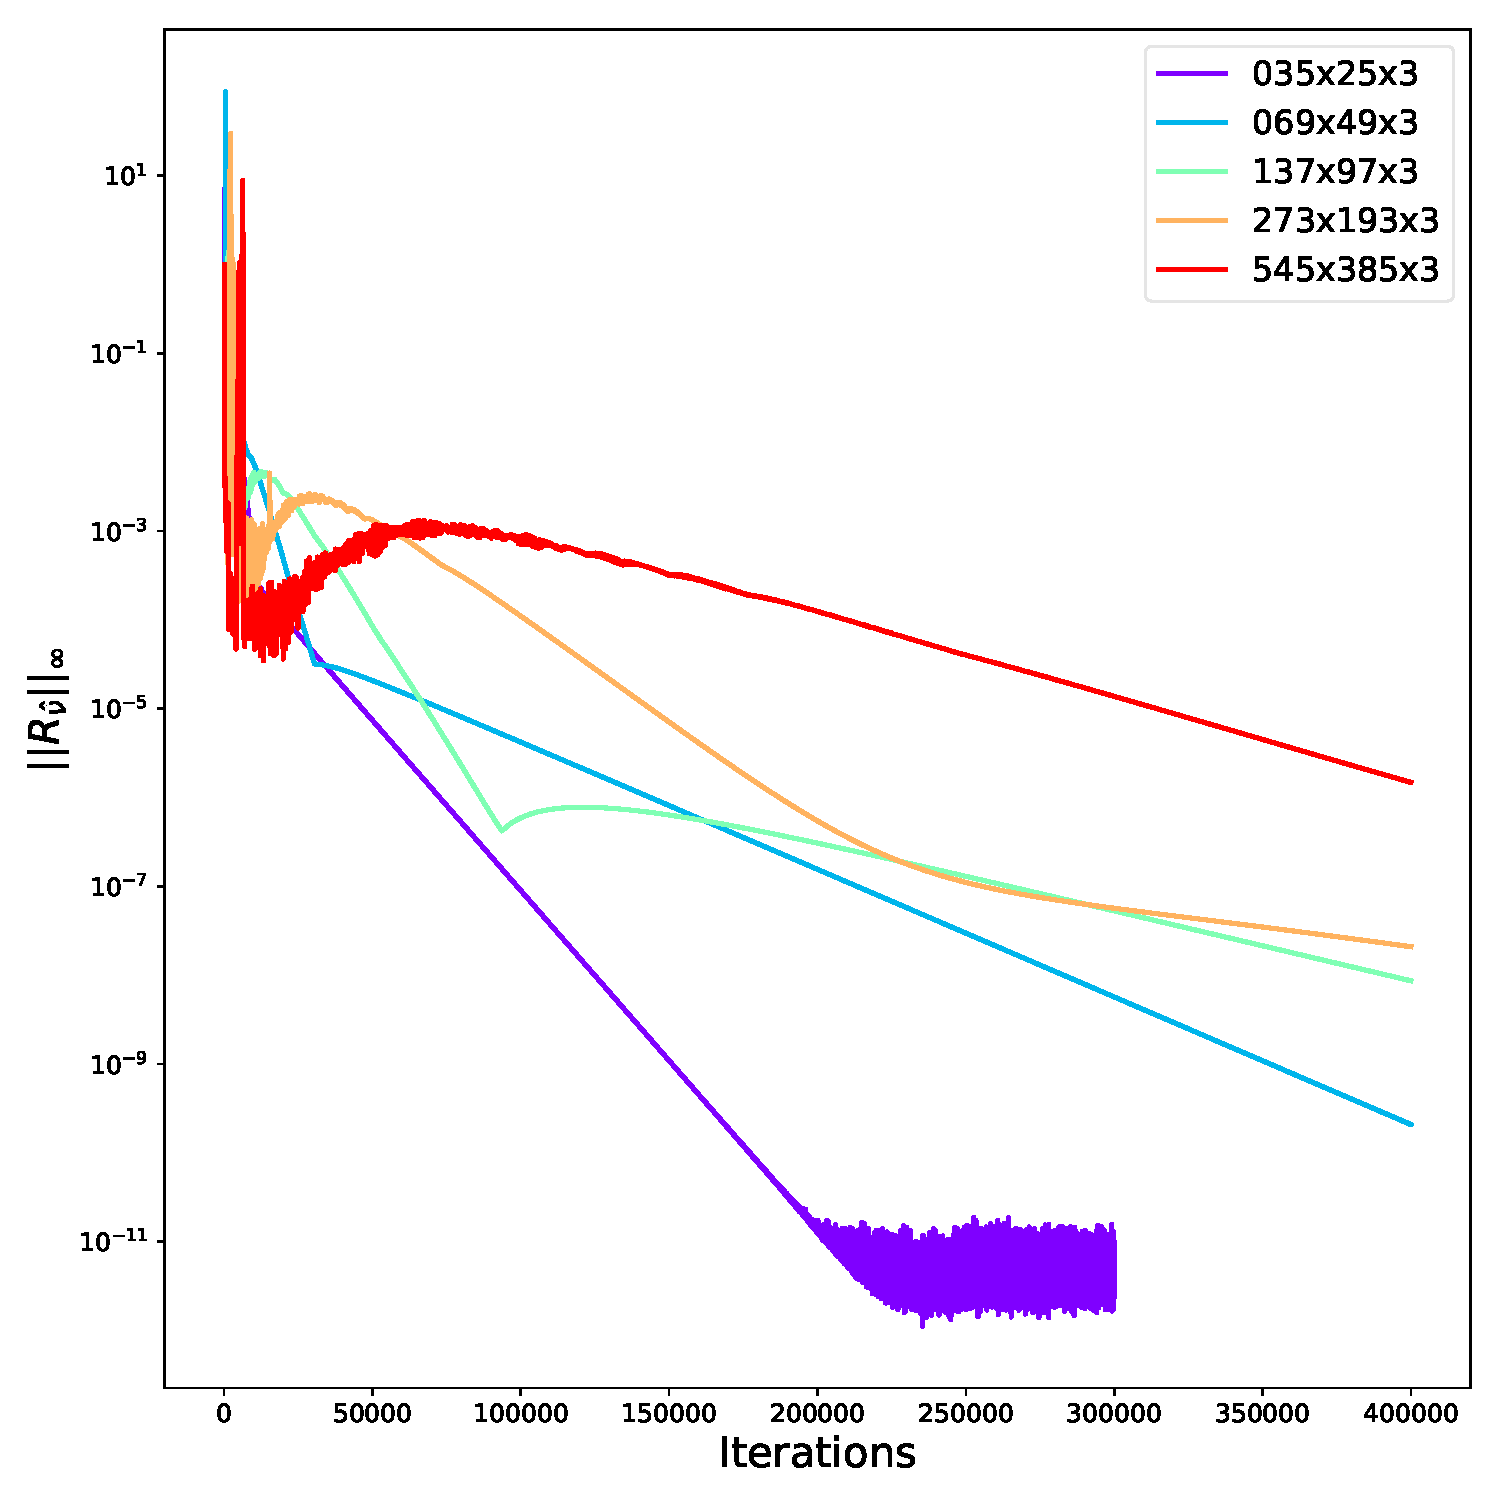
\includegraphics[width=1.0\textwidth]{figs/flat/SA_convergence_gridstudy.pdf}
    \caption{Maximum turbulence variable residual.}
\end{subfigure}
\caption{Flat Plate (Syn3D): Convergence of flow and turbulence variables on various grid sizes.}
\label{fig:synflatcnvstudy}
\end{figure}
% \begin{figure}[ht!]
% \centering
% \begin{subfigure}{.45\textwidth}
%   \centering
%   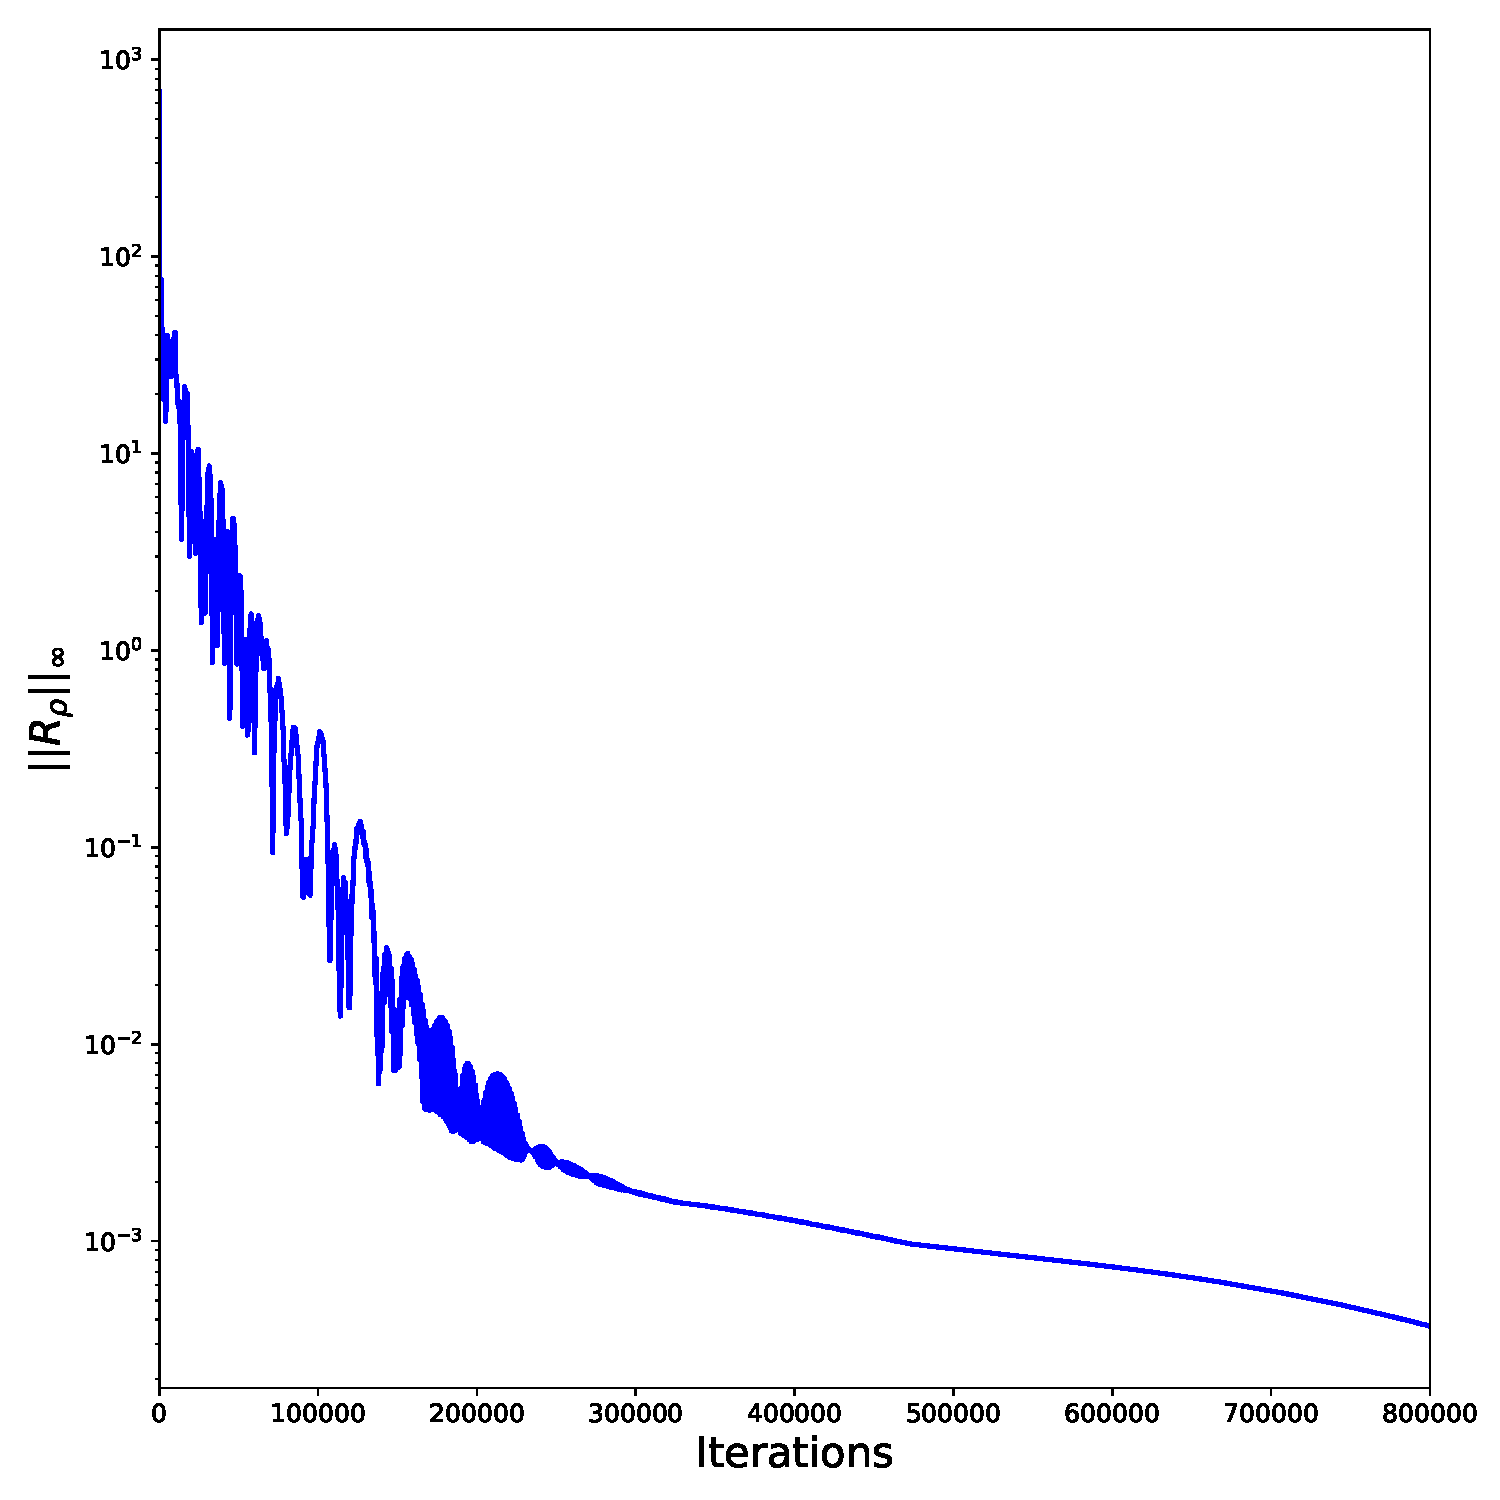
\includegraphics[width=1.0\textwidth]{figs/flat/gov_convergence.pdf}
%   \caption{Maximum density residual}
% \end{subfigure}%
% \begin{subfigure}{.45\textwidth}
%   \centering
%   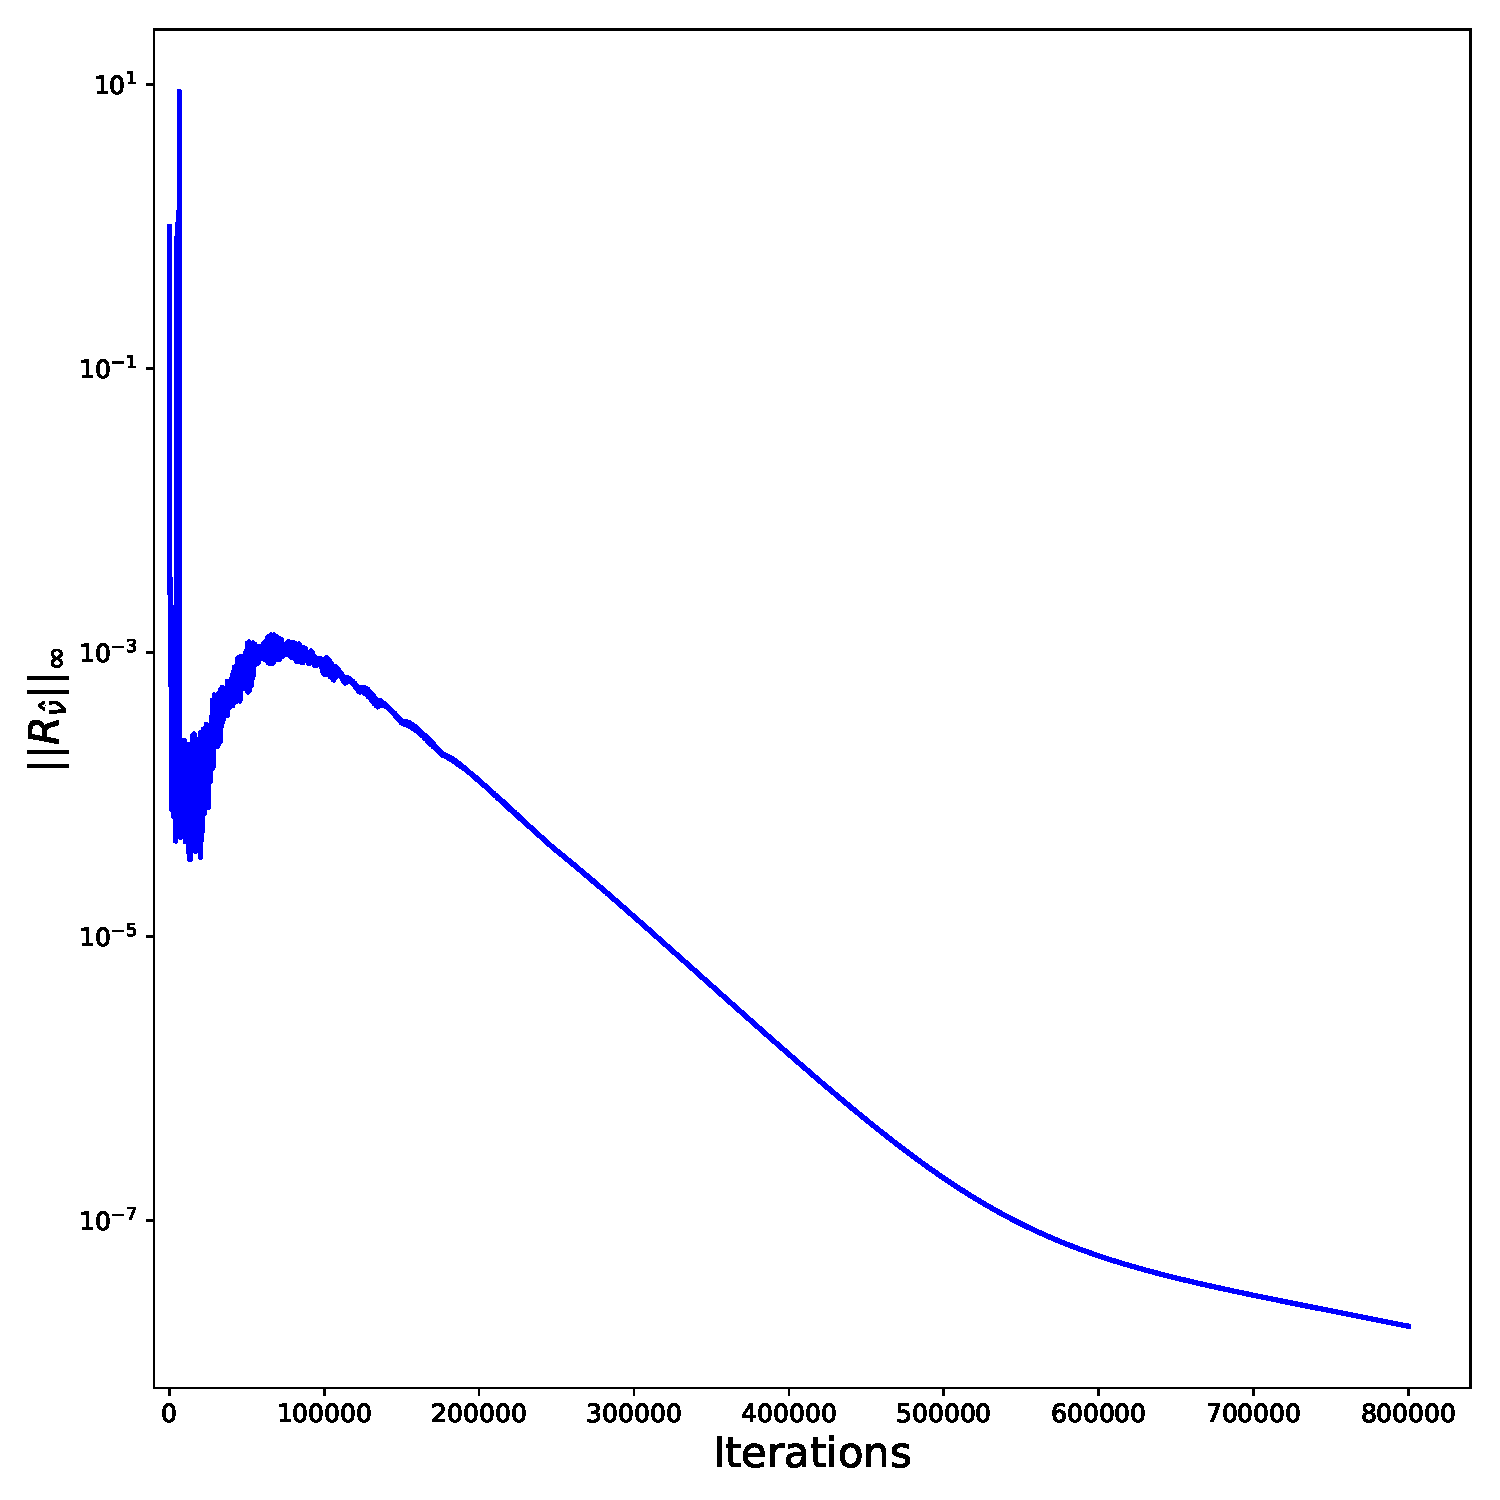
\includegraphics[width=1.0\textwidth]{figs/flat/turb_convergence.pdf}
%   \caption{Maximum turbulent variable residuals}
% \end{subfigure}
% \caption{Convergence of flow and turbulence variables (finest flat plate).}
% \label{fig:synflatcnv}
% \end{figure}

Several plots have been generated to compare the results between Syn3D and CFL3D. Unless otherwise noted, all results were obtained with the finest grid. \Cref{fig:synflatcf} compares the skin friction along the plate. \Cref{fig:synflatmutcontour} shows contour plots of the dimensionless eddy viscosity $\frac{\mu_t}{\mu_{\infty}}$ and \Cref{fig:synflatmu} shows line plots of the dimensionless eddy viscosity. \Cref{fig:synflatu,fig:synflatupyp} show profiles of the dimensionless velocity $u/u_\infty$ and $u^+$ respectively. There is decent agreement between the two solvers, and the source of discrepancy is easily seen in~\Cref{fig:synflatmutmax}: the eddy viscosity jumps abruptly right at the leading edge for Syn3D but not for CFL3D. The cause of this jump was investigated by the author as well as others working on the code, but a definite answer was unfortunately not found.
\begin{figure}[ht!]
\centering
	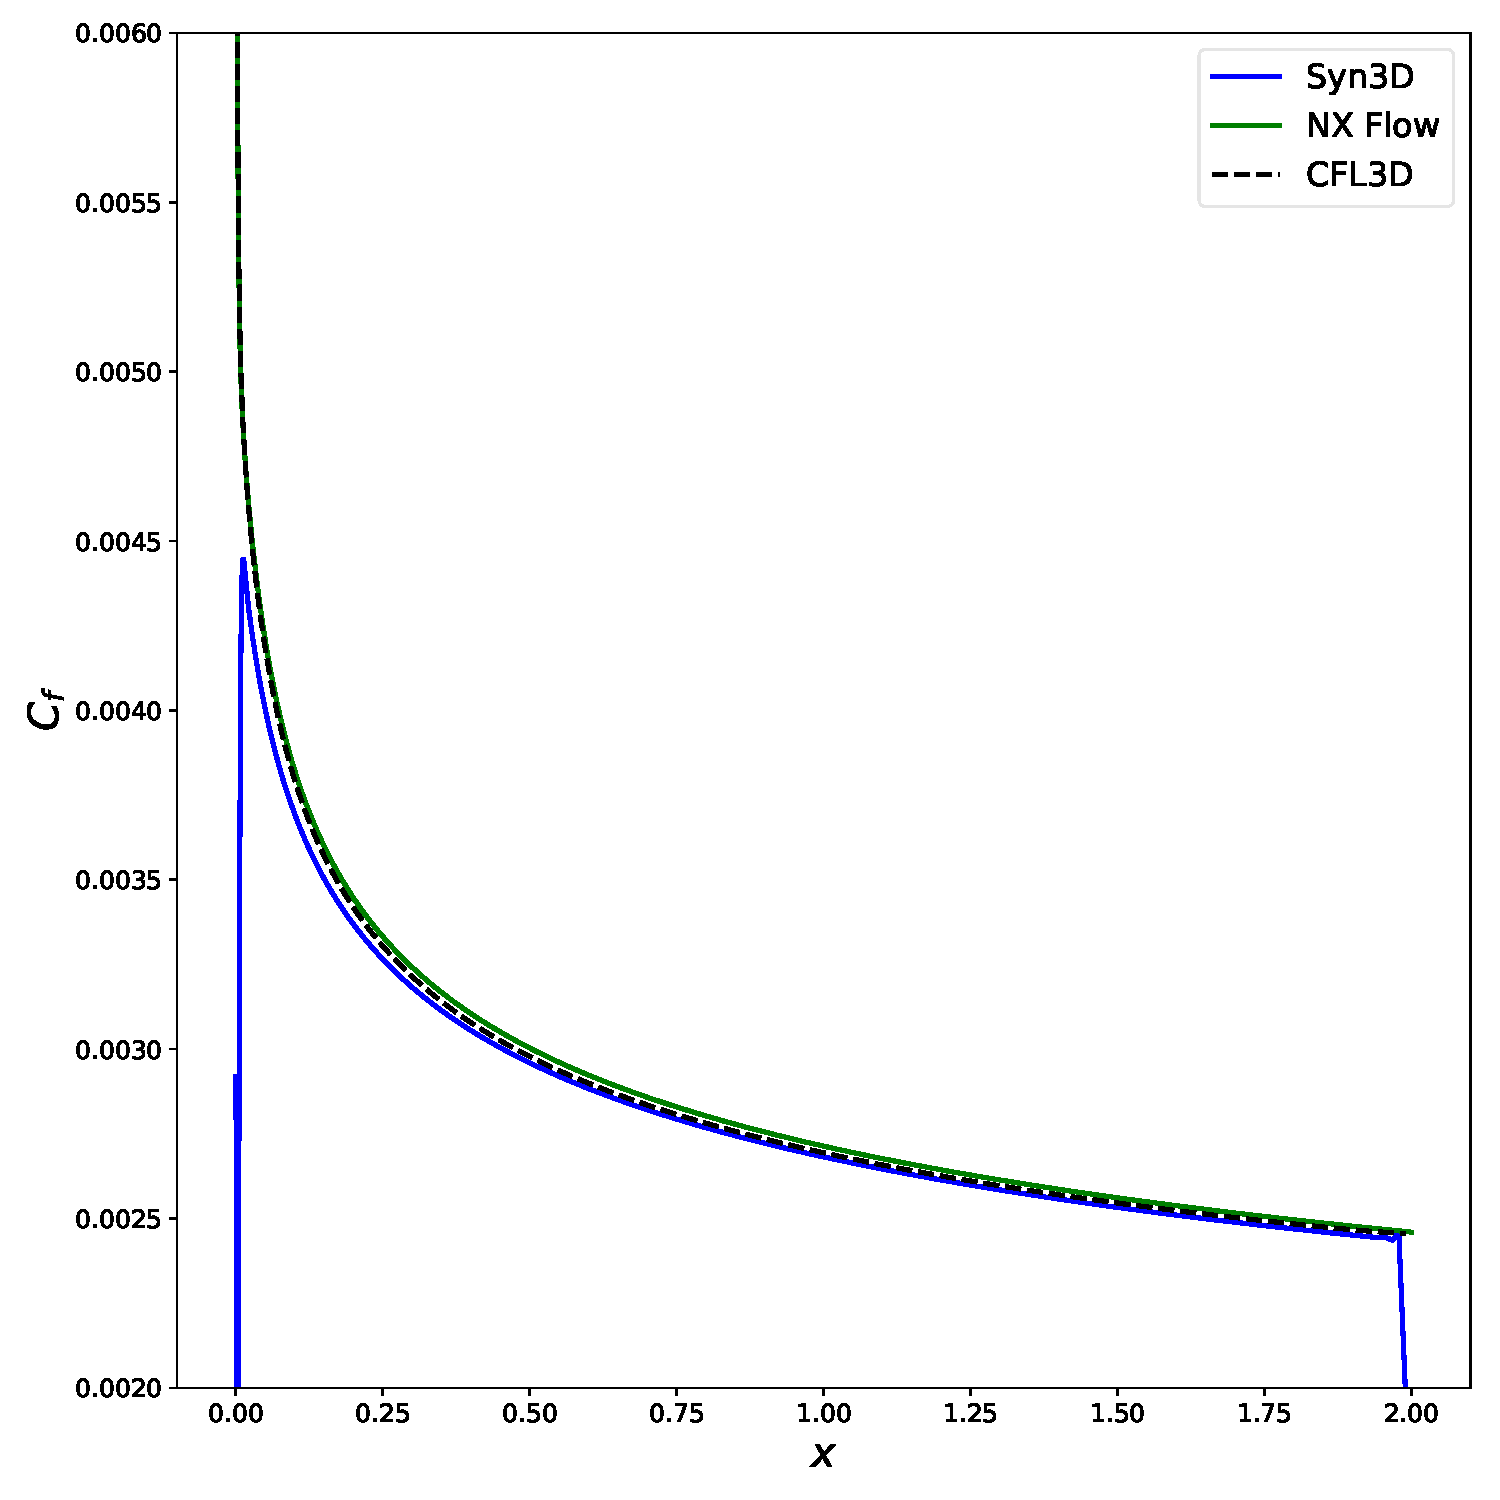
\includegraphics[width=0.7\textwidth]{figs/flat/skin_friction.pdf}
    \caption{Flat Plate (Syn3D): Coefficient of skin friction along the plate.}
    \label{fig:synflatcf}
\end{figure}

\begin{figure}[ht!]
\centering
\begin{subfigure}{.45\textwidth}
  \centering
  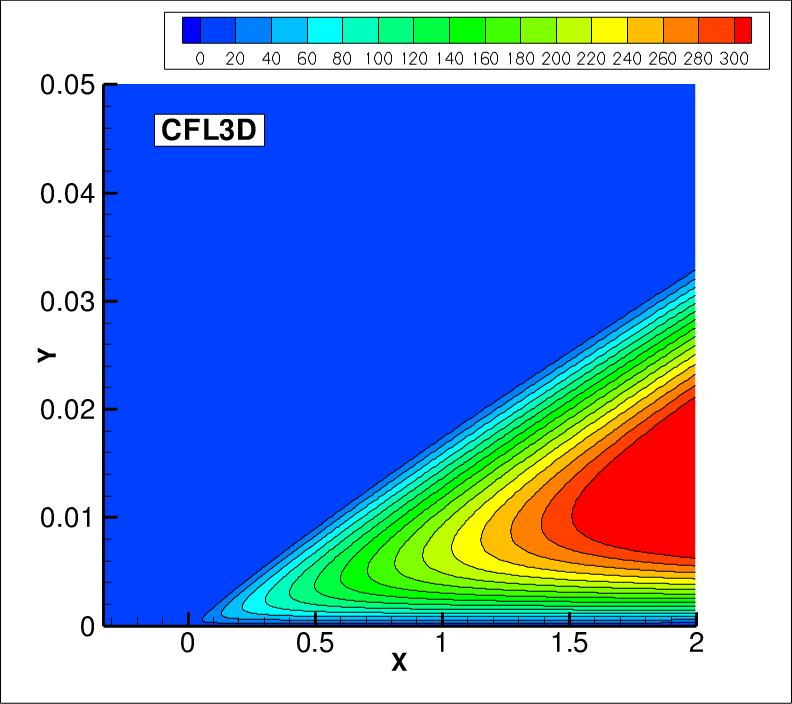
\includegraphics[width=1.0\textwidth]{figs/flat/mut_contours_cfl3d.jpg}
  \caption{CFL3D}
\end{subfigure}%
\begin{subfigure}{.45\textwidth}
  \centering
  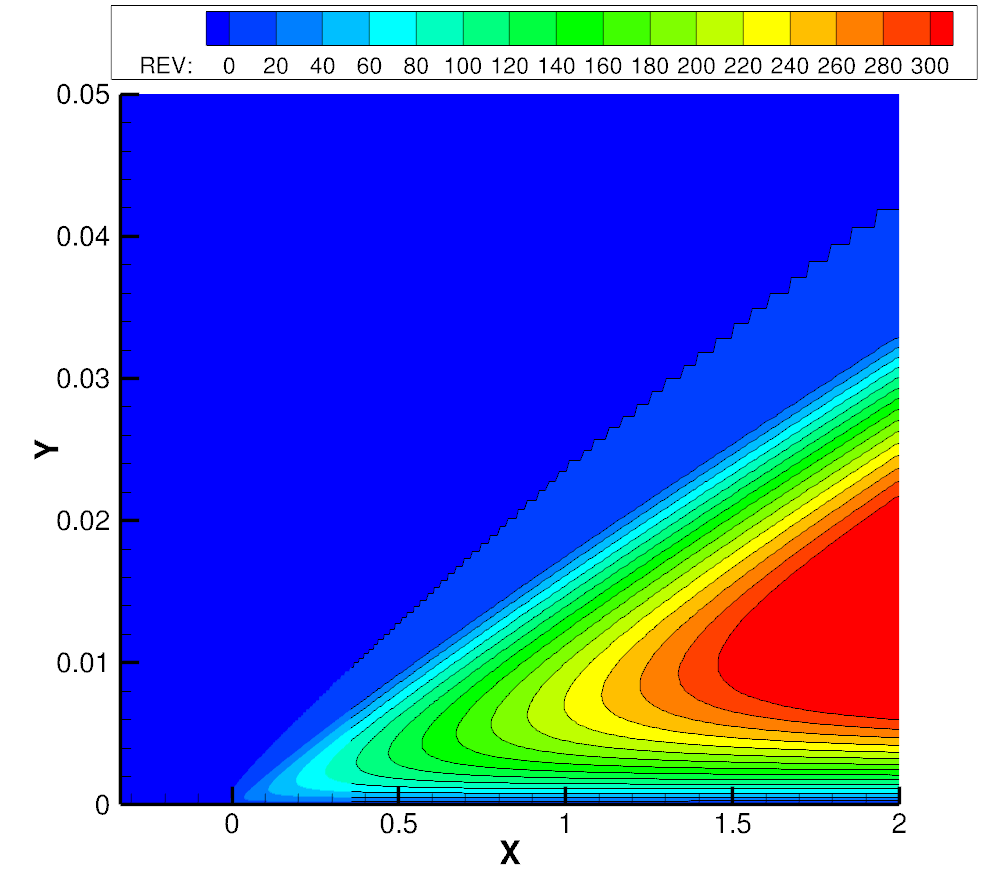
\includegraphics[width=1.0\textwidth]{figs/flat/rev_sa.png}
  \caption{Syn3D}
\end{subfigure}
\caption{Flat Plate (Syn3D): Contours of non-dimensionalized eddy viscosity}
\label{fig:synflatmutcontour}
\end{figure}

\begin{figure}[ht!]
\centering
\begin{subfigure}{.45\textwidth}
  \centering
  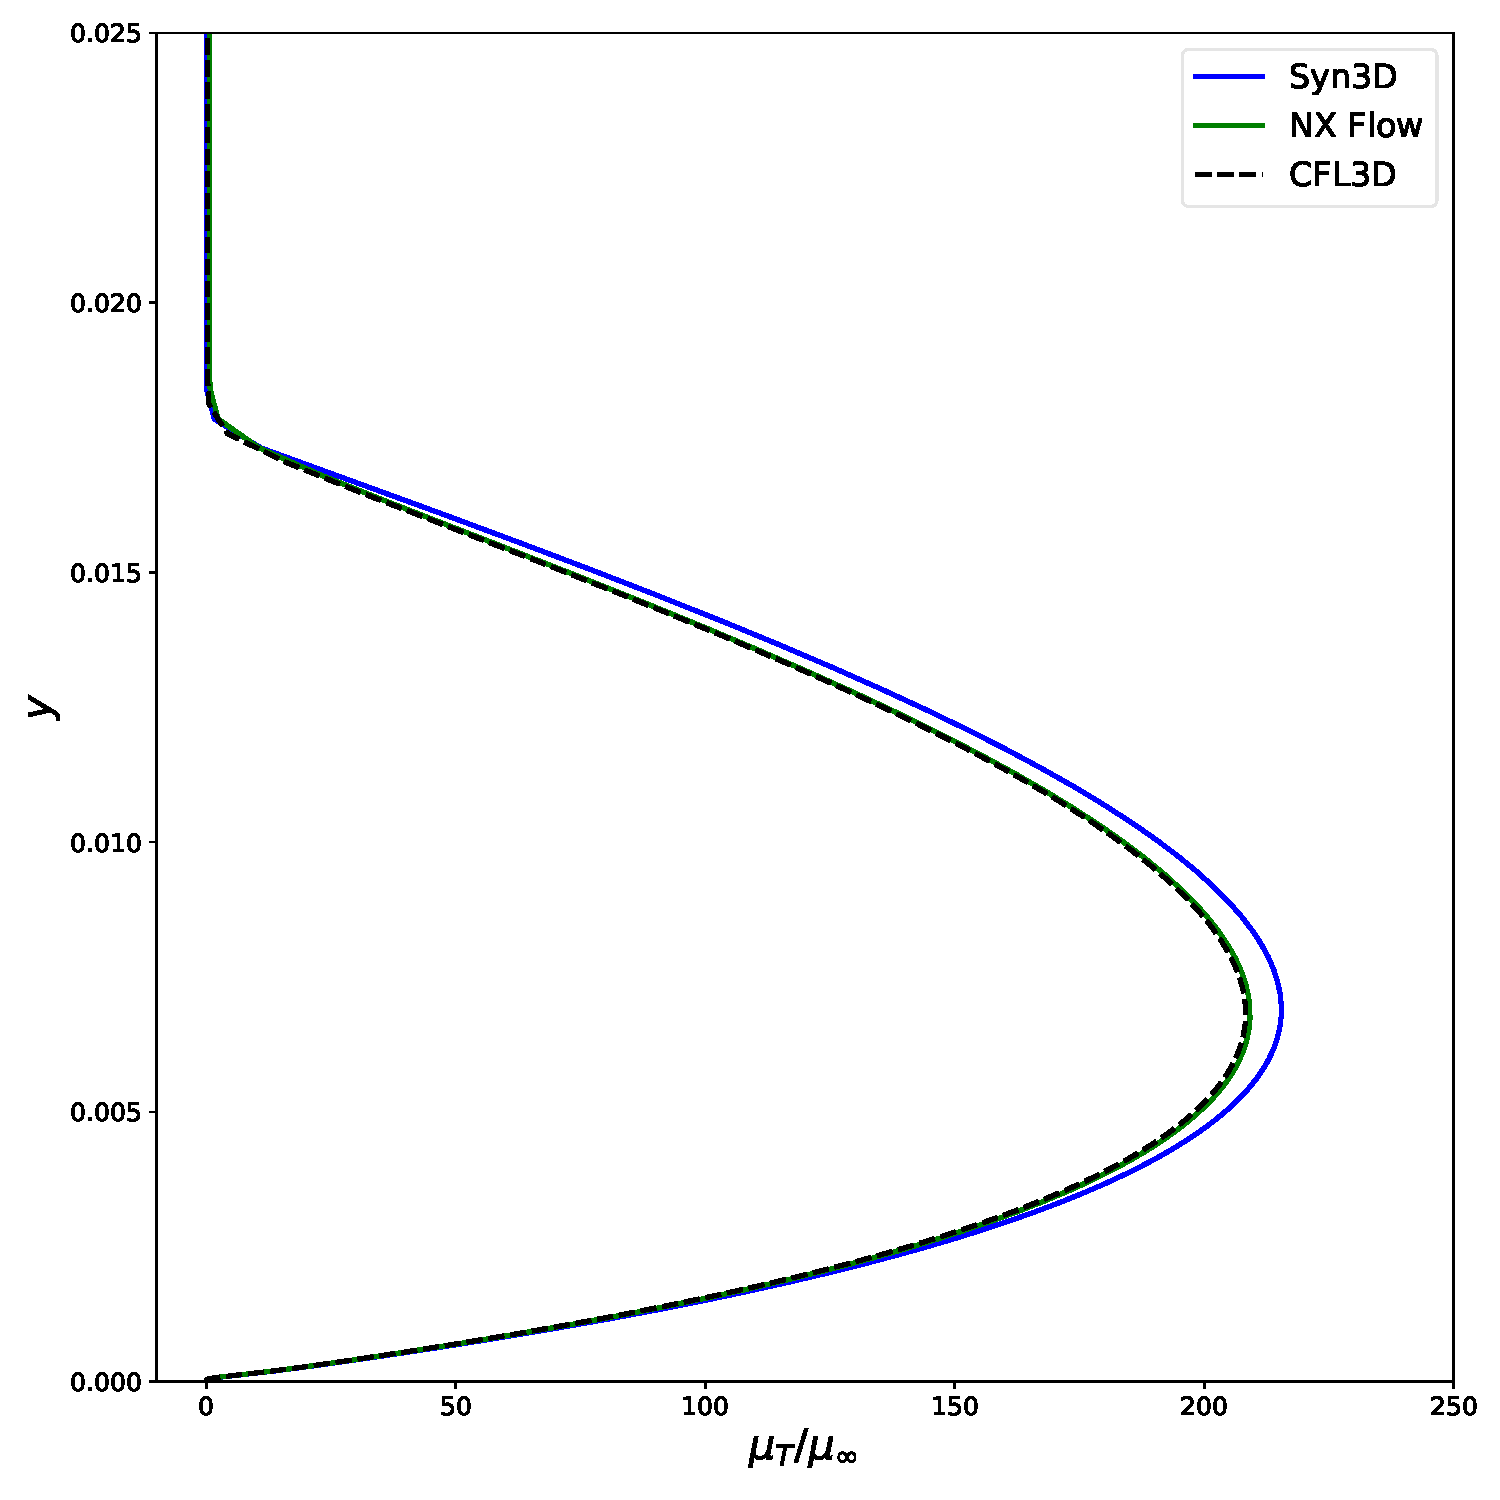
\includegraphics[width=1.0\textwidth]{figs/flat/mut_x097.pdf}
  \caption{Nondimensional eddy viscosity at x=0.97 }
\end{subfigure}%
\begin{subfigure}{.45\textwidth}
  \centering
  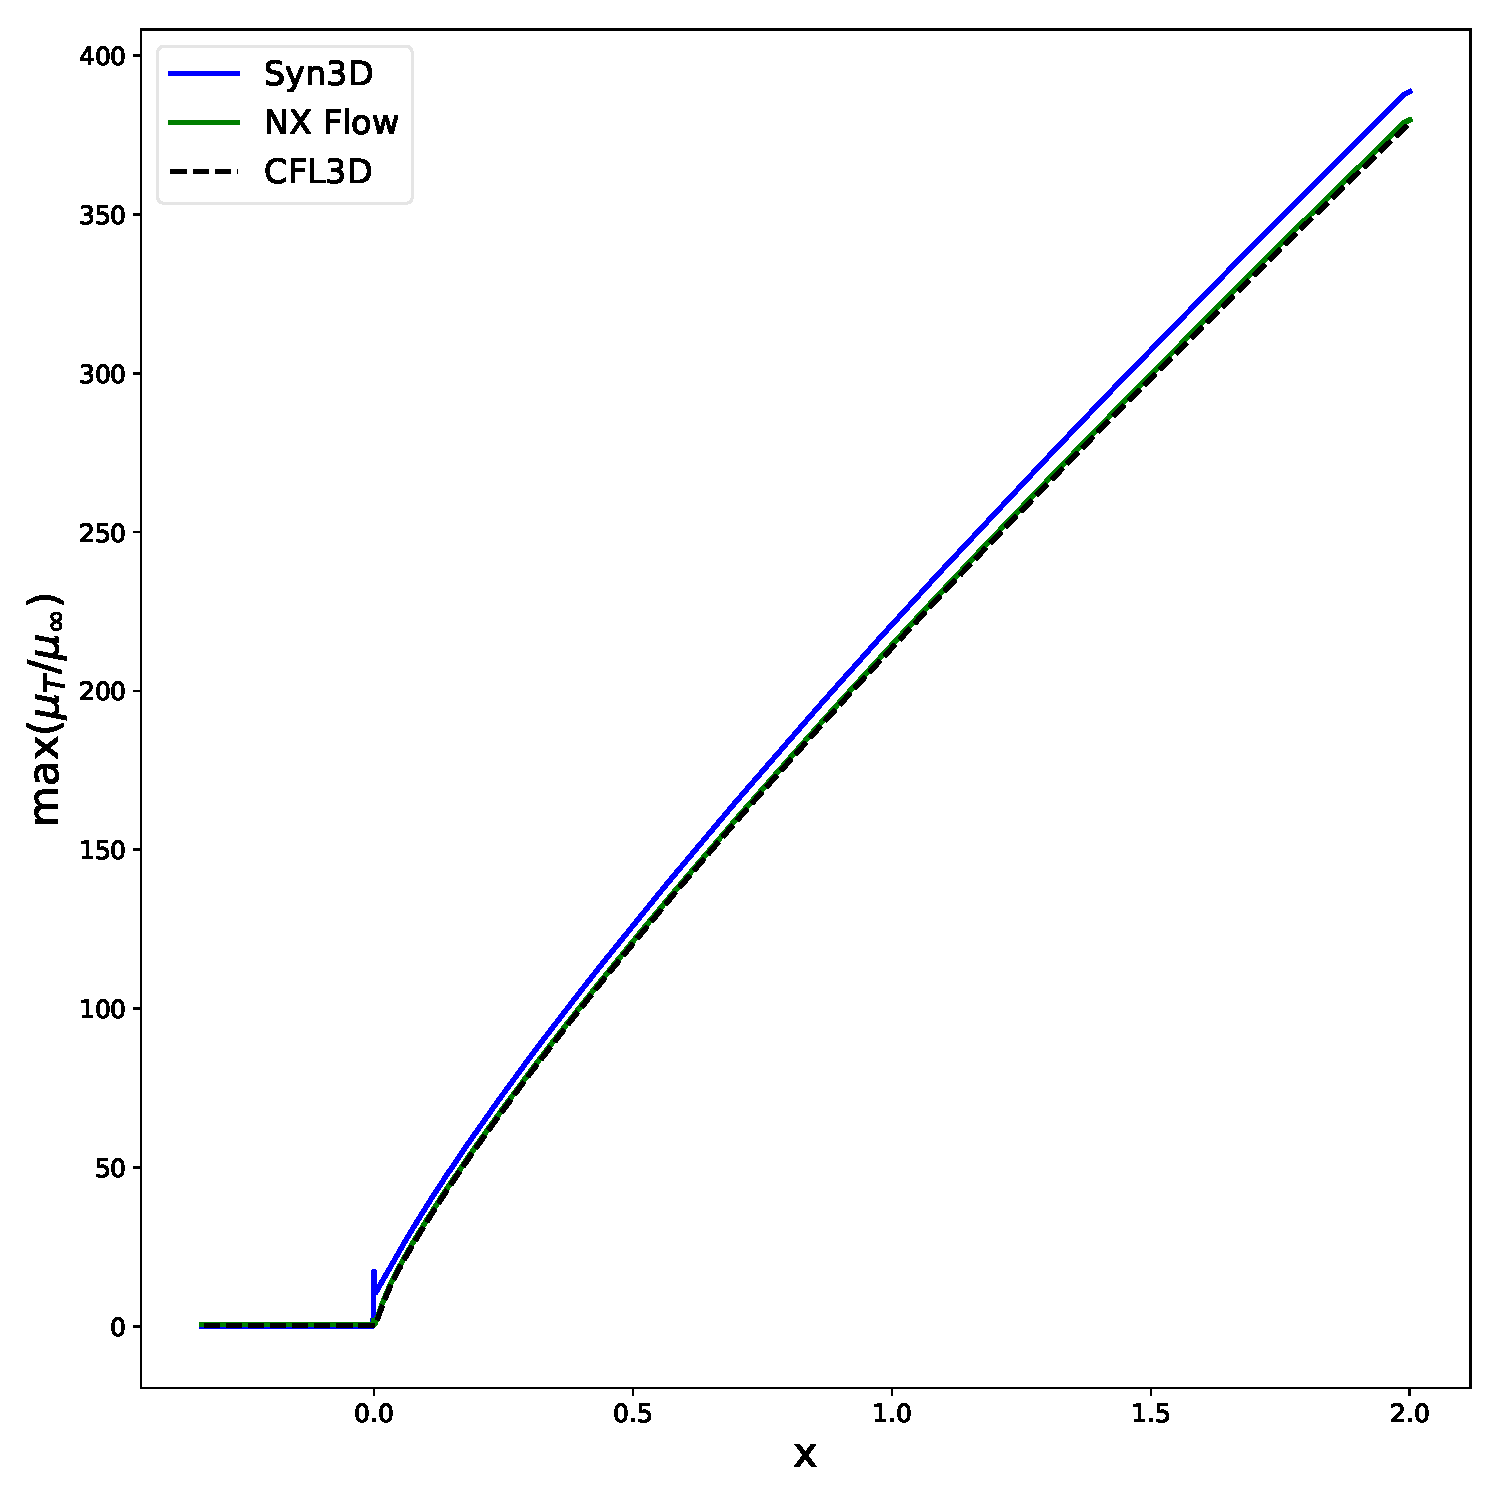
\includegraphics[width=1.0\textwidth]{figs/flat/maxmut.pdf}
  \caption{Maximum $\frac{\mu_t}{\mu_{\infty}}$ in the boundary layer}
  \label{fig:synflatmutmax}
\end{subfigure}
\caption{Flat Plate (Syn3D): Dimensionless eddy viscosity line plots}
\label{fig:synflatmu}
\end{figure}

\begin{figure}[ht!]
\centering
\begin{subfigure}{.45\textwidth}
  \centering
  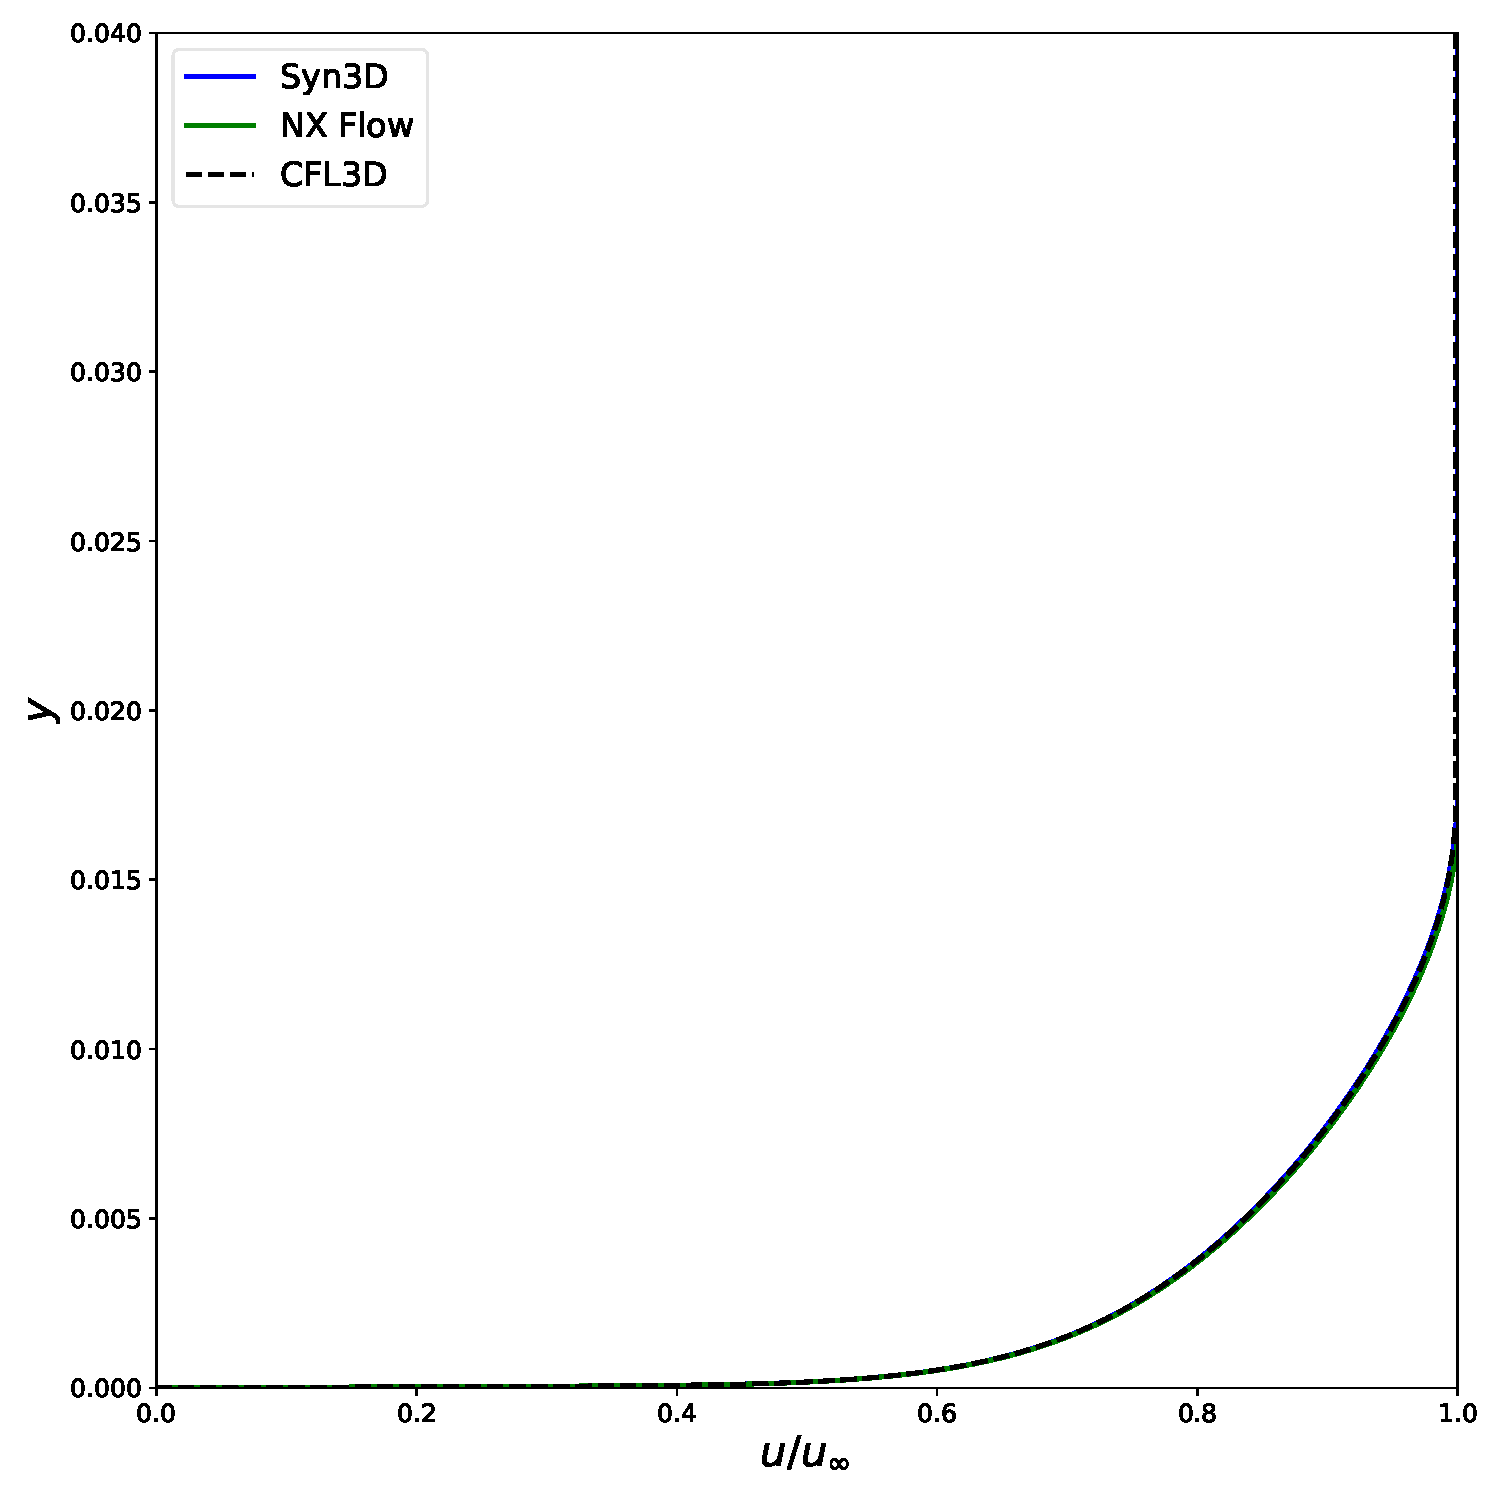
\includegraphics[width=1.0\textwidth]{figs/flat/u097.pdf}
  \caption{$x=0.97$}
\end{subfigure}%
\begin{subfigure}{.45\textwidth}
  \centering
  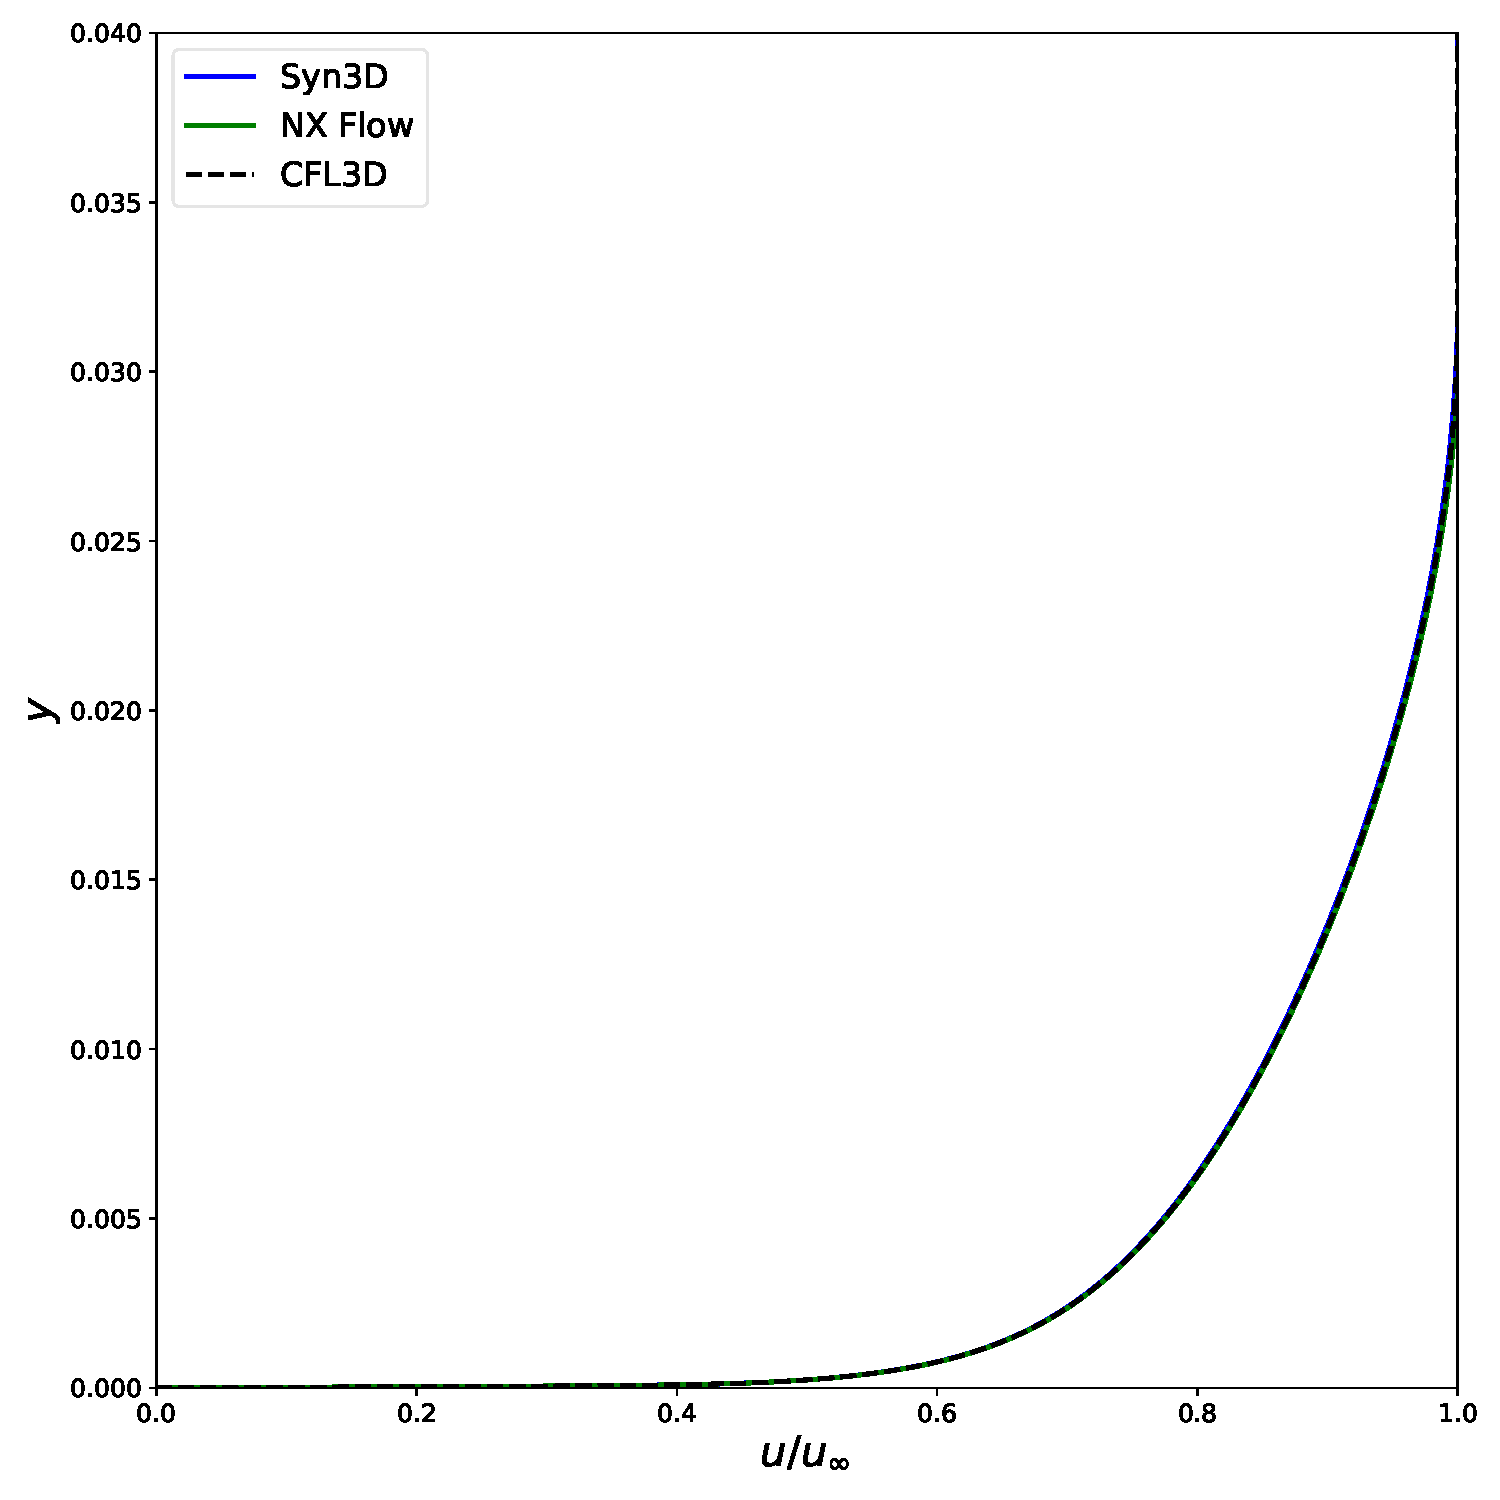
\includegraphics[width=1.0\textwidth]{figs/flat/u190.pdf}
  \caption{$x=1.90$}
\end{subfigure}
\caption{Flat Plate (Syn3D): $\frac{U}{U_{\infty}}$ profiles in the boundary layer}
\label{fig:synflatu}
\end{figure}

\begin{figure}[ht!]
\centering
\begin{subfigure}{.45\textwidth}
  \centering
  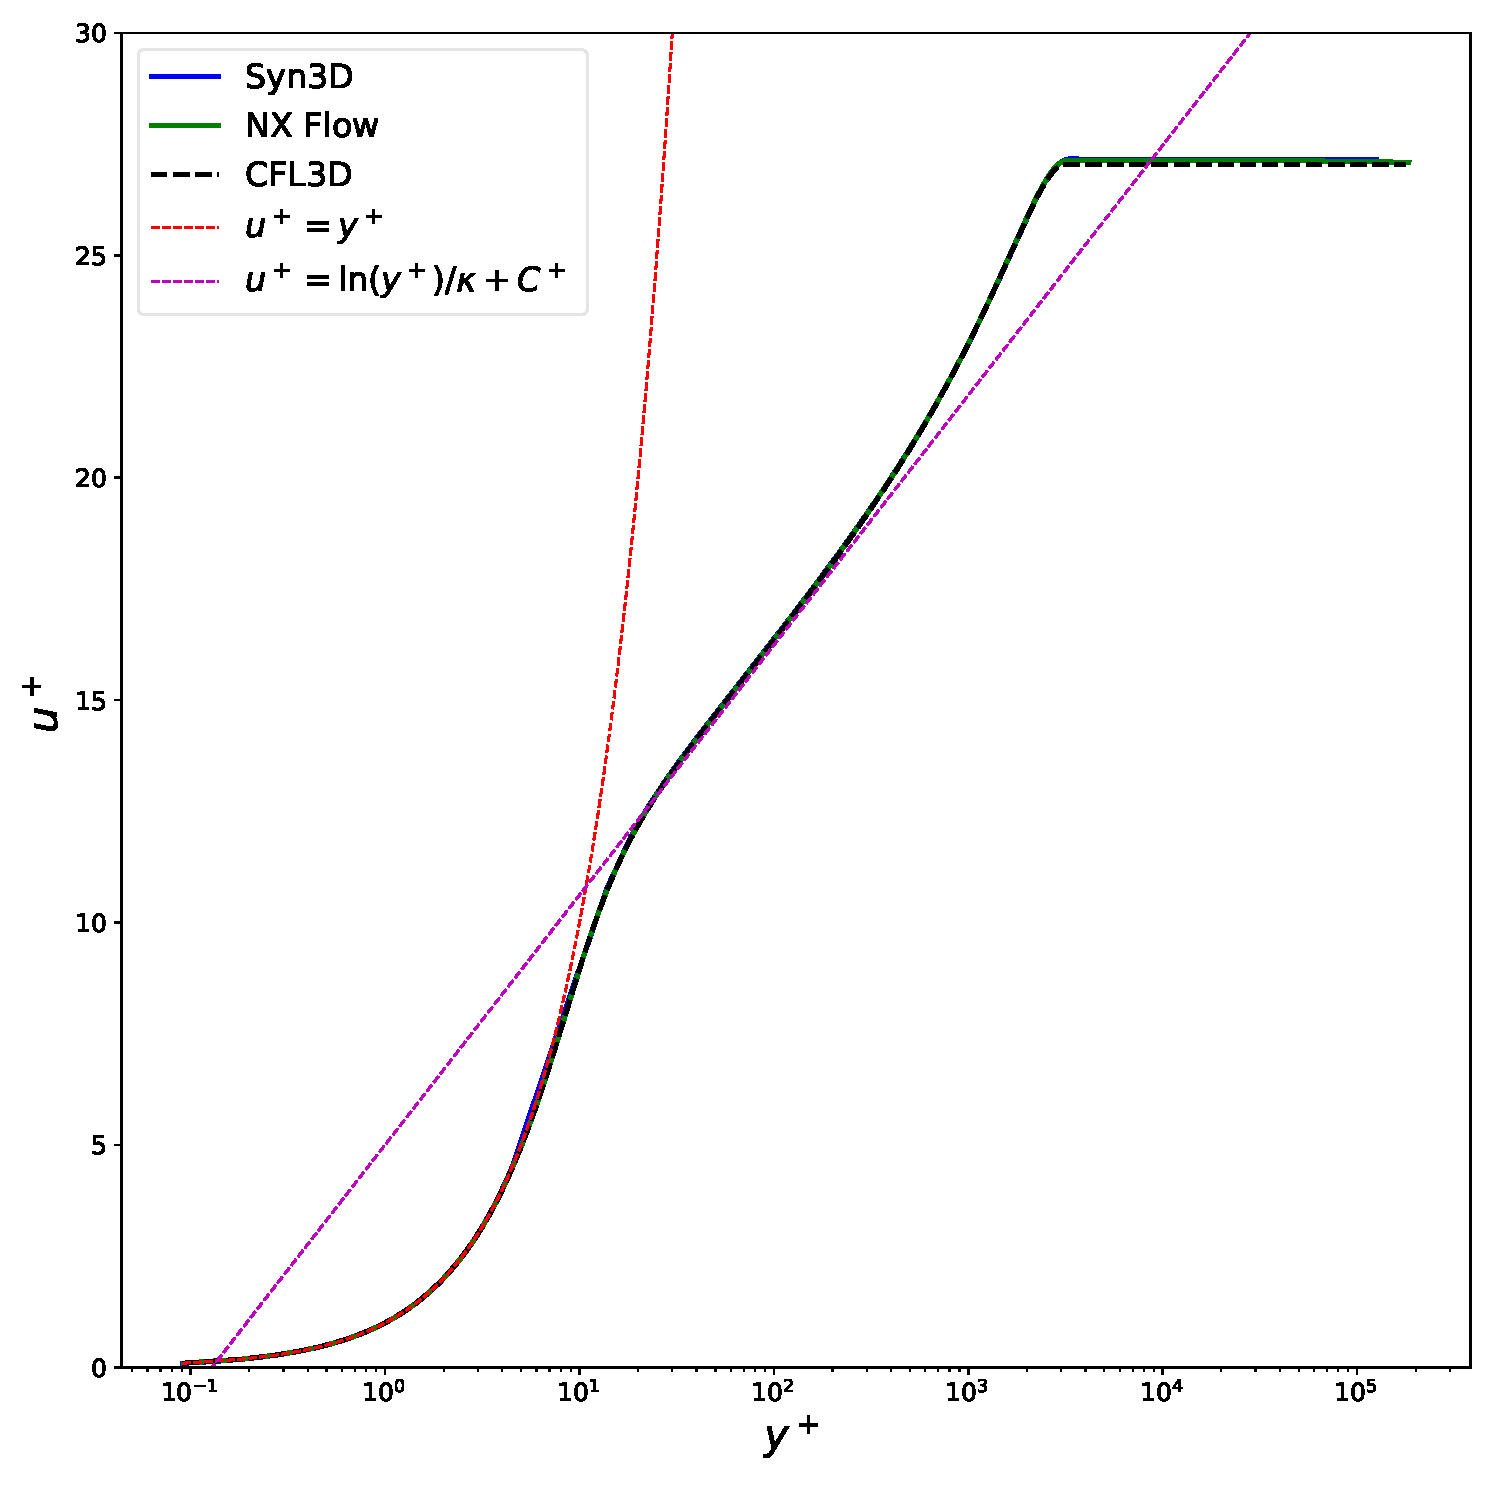
\includegraphics[width=1.0\textwidth]{figs/flat/uplus_yplus_097.pdf}
  \caption{$x=0.97$}
\end{subfigure}%
\begin{subfigure}{.45\textwidth}
  \centering
  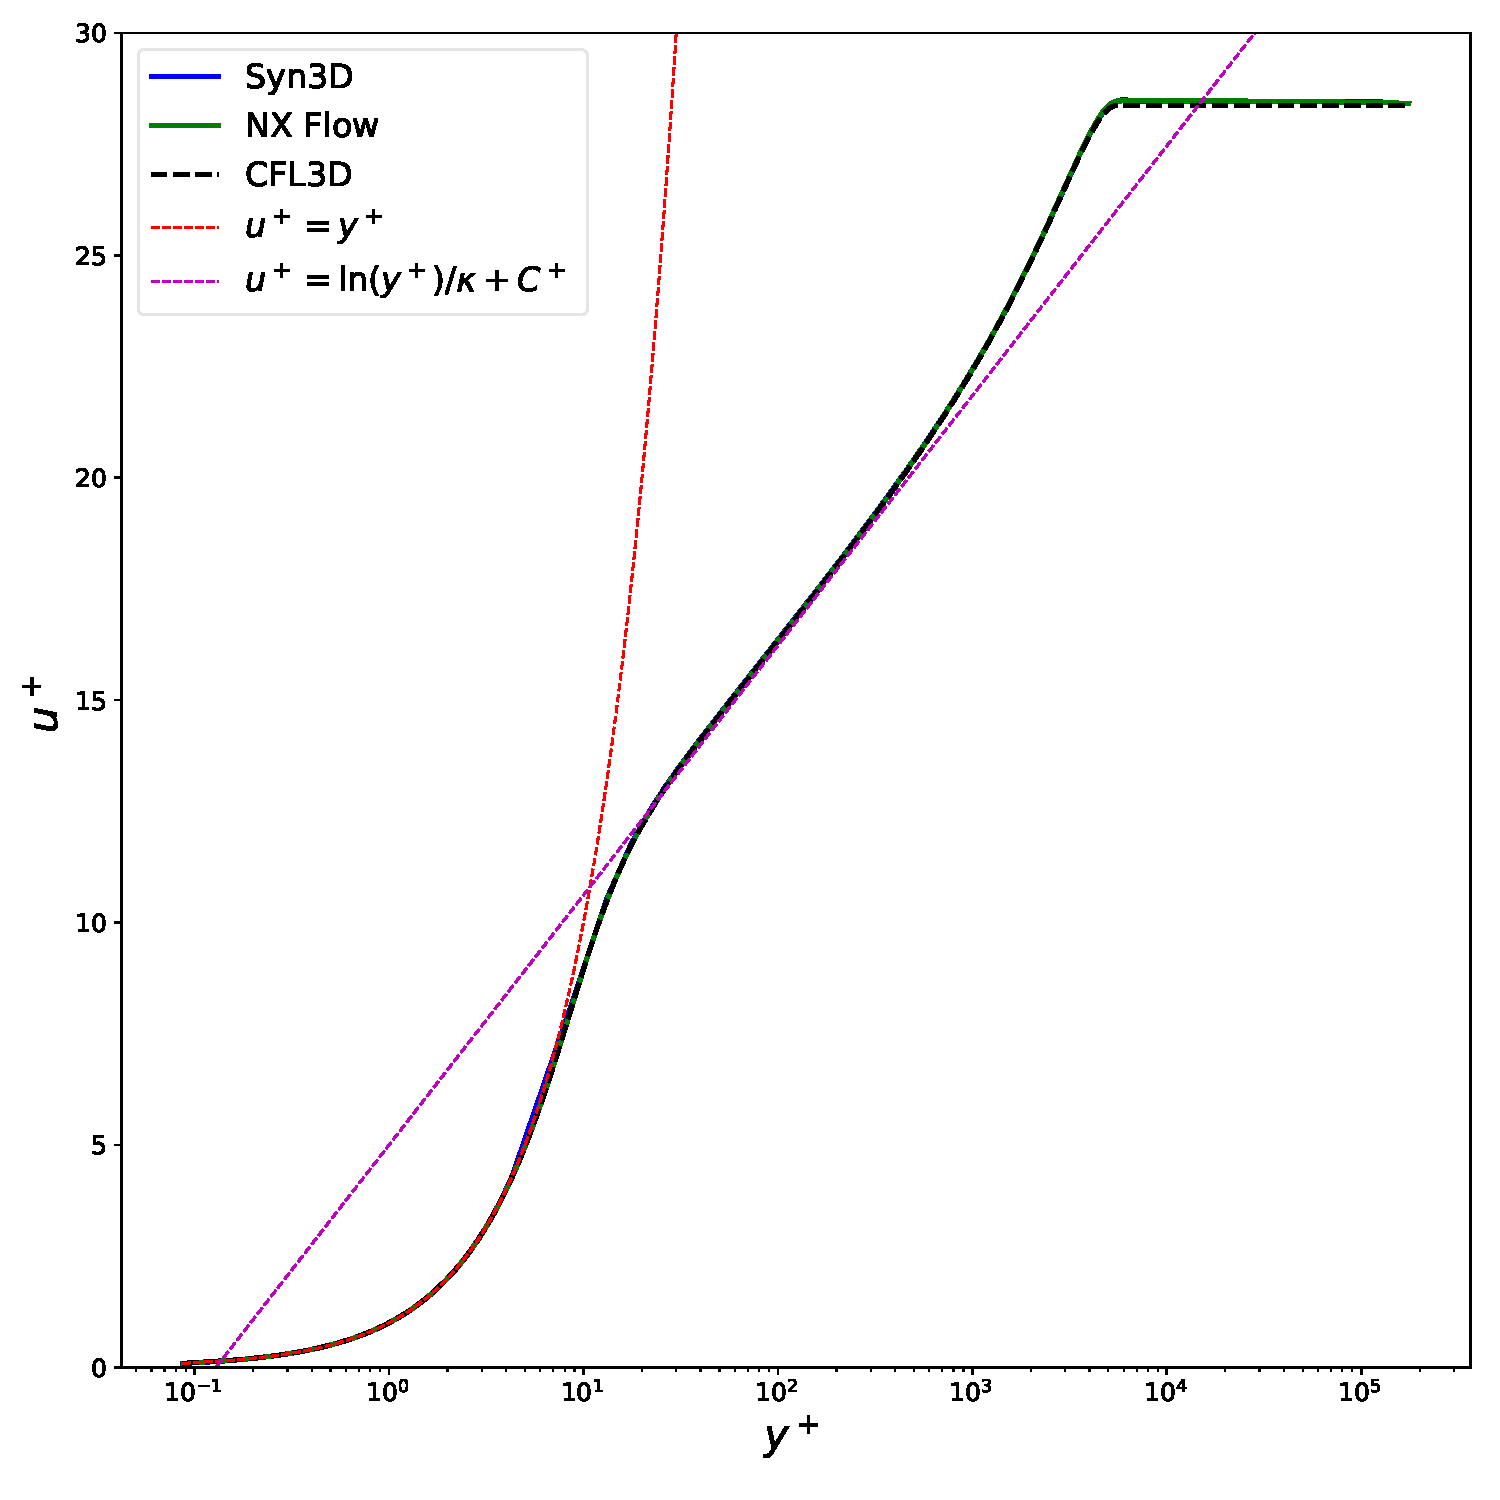
\includegraphics[width=1.0\textwidth]{figs/flat/uplus_yplus_190.pdf}
  \caption{$x=1.90$}
\end{subfigure}
\caption{Flat Plate (Syn3D): $u^+$ vs. $y^+$ profiles in the boundary layer. Law of the wall is also shown for comparison.}
\label{fig:synflatupyp}
\end{figure}

Next, \Cref{fig:synflatforcestudy} shows the dependence of $C_D$ and $C_f$ on the grid spacing $h = 1/N^2$, where $N$ is the number of grid points. It can be seen that there is still significant differences in results between the second finest and finest grid for Syn3D as compared to CFL3D and FUN3D -- the latter is a vertex-centered code also developed by NASA. \Cref{fig:synflatcnvstudy} shows the Syn3D convergence of residuals for all five grids. As expected, the coarser grids show faster convergence than the finer ones -- this phenomenon is detailed in~\cite{blazek2015computational}. \Cref{fig:synflatcfstudy,fig:synflatprofilestudy} show the variation of skin friction coefficient along the plate and profiles of eddy viscosity and velocity with grid size respectively. These plots show that the solution field seems to converge to a unique solution, as opposed to oscillating back and forth between different values.
\begin{figure}[ht!]
\centering
\begin{subfigure}{.45\textwidth}
  \centering
  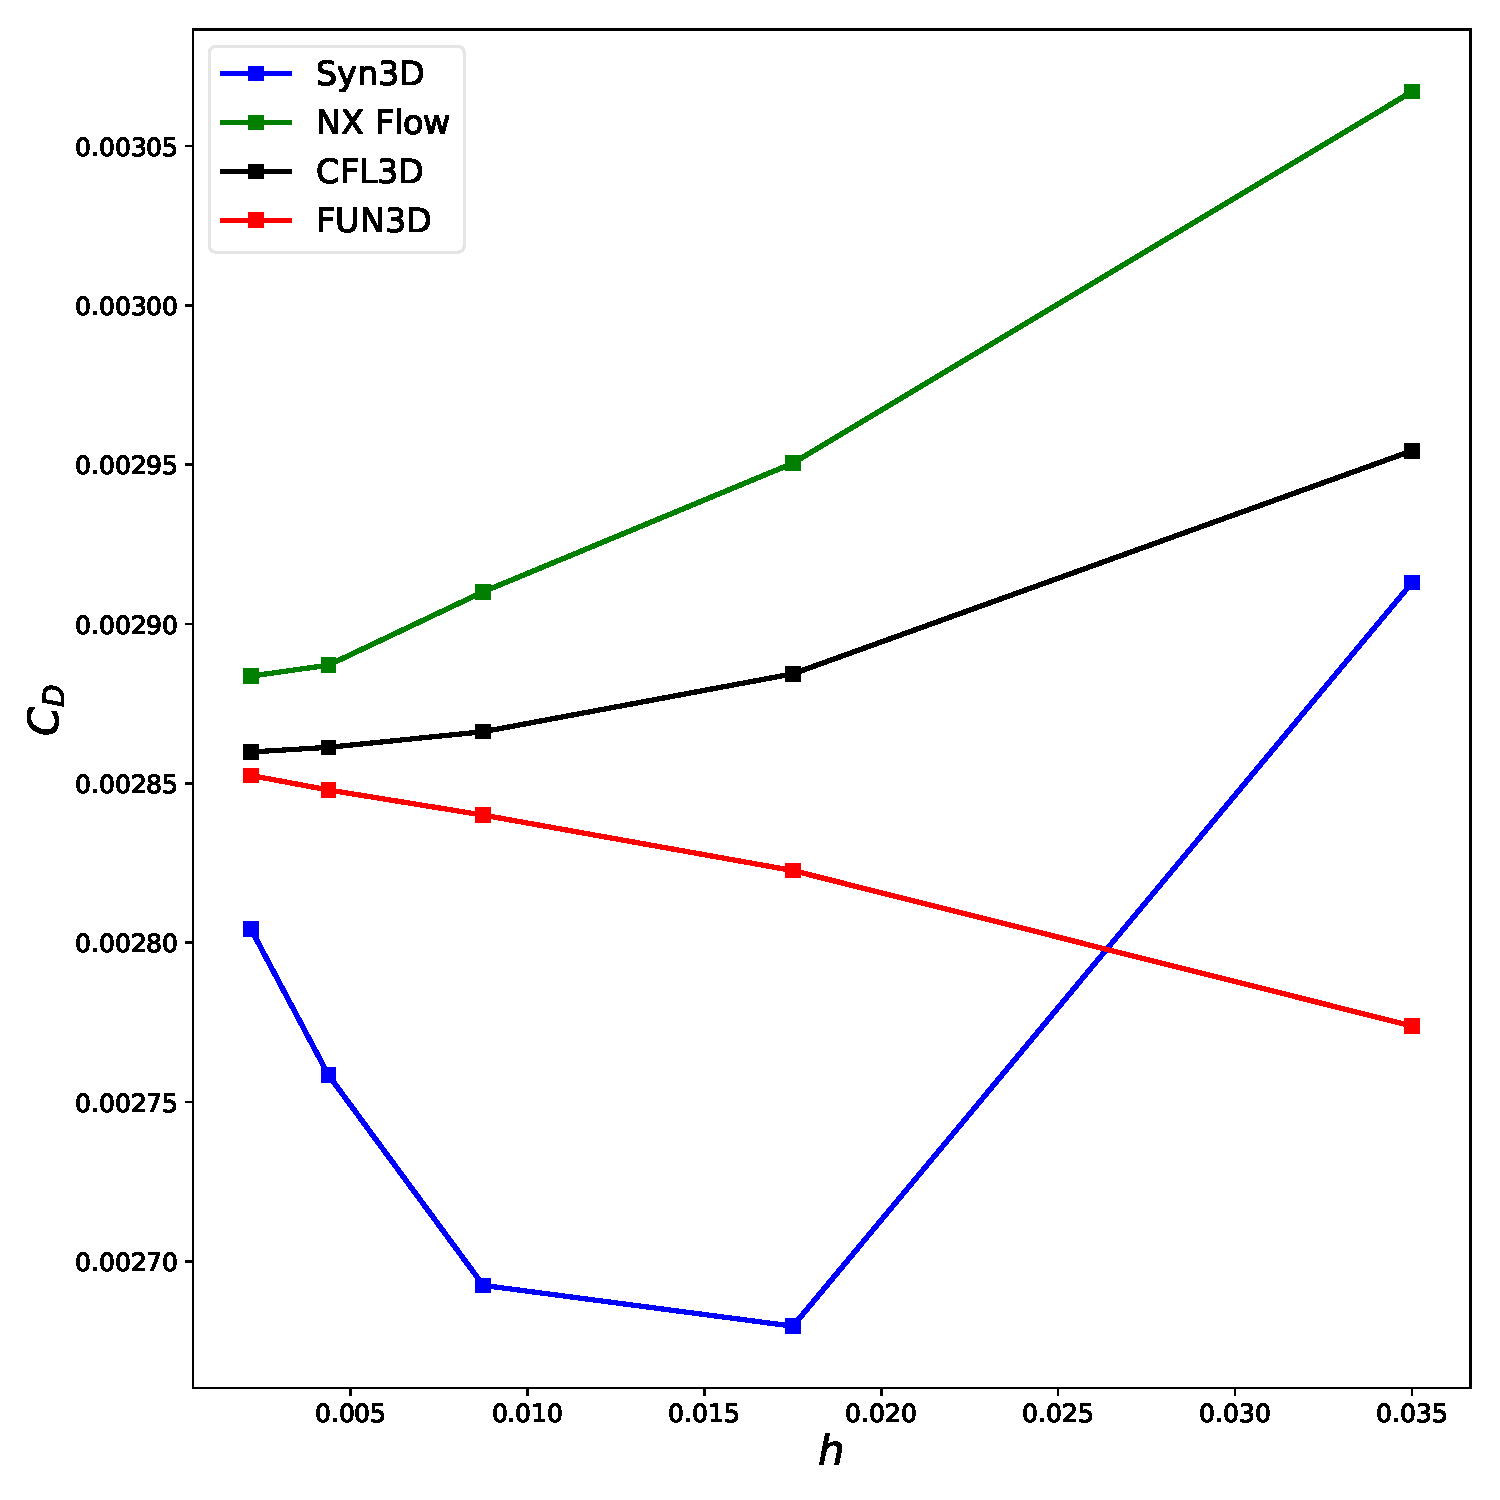
\includegraphics[width=1.0\textwidth]{figs/flat/cd_grid.pdf}
  \caption{Coefficient of drag.}
\end{subfigure}%
\begin{subfigure}{.45\textwidth}
  \centering
  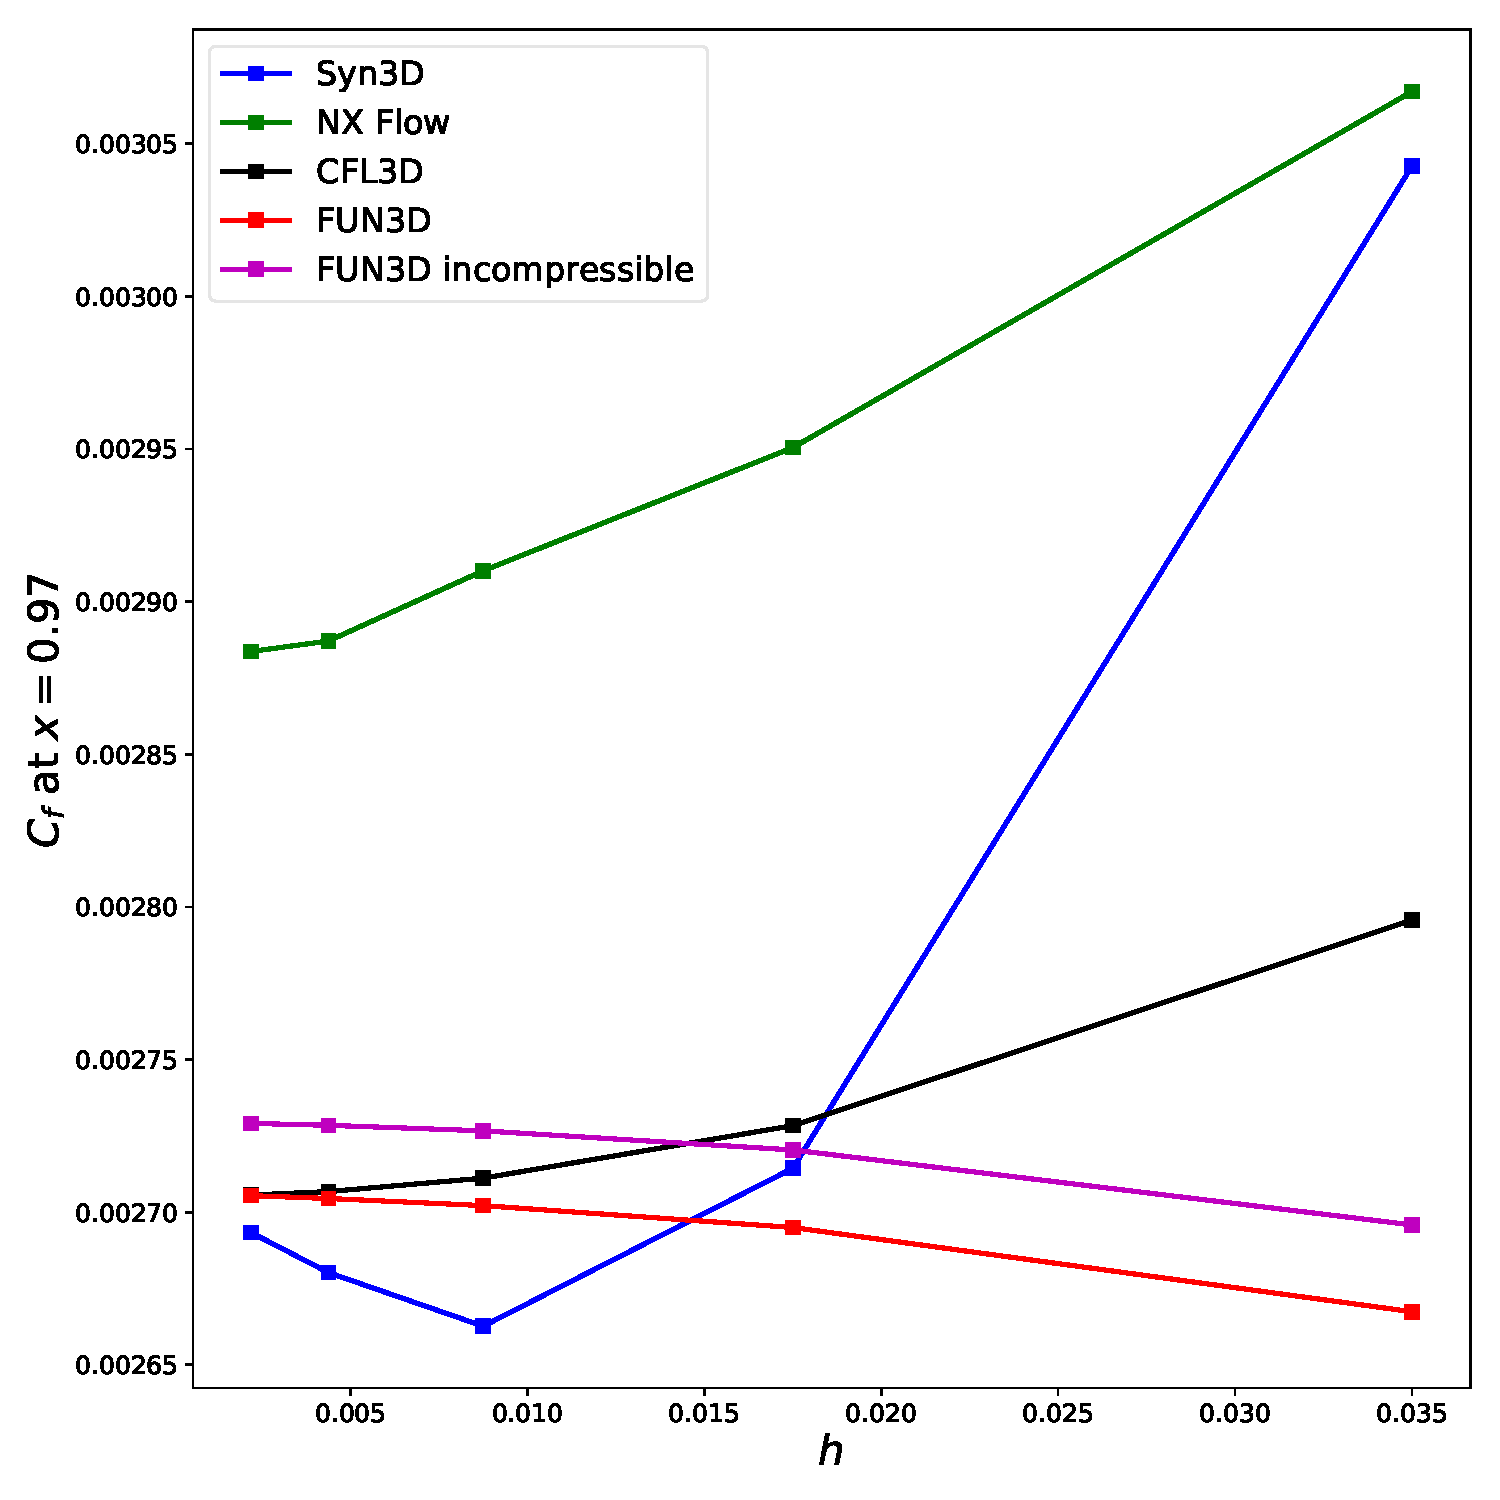
\includegraphics[width=1.0\textwidth]{figs/flat/cf_grid.pdf}
  \caption{Coefficient of Skin Friction at x=0.97.}
\end{subfigure}
\caption{Flat Plate (Syn3D): Force coefficients for various grid sizes.}
\label{fig:synflatforcestudy}
\end{figure}

\begin{figure}[ht!]
\centering
  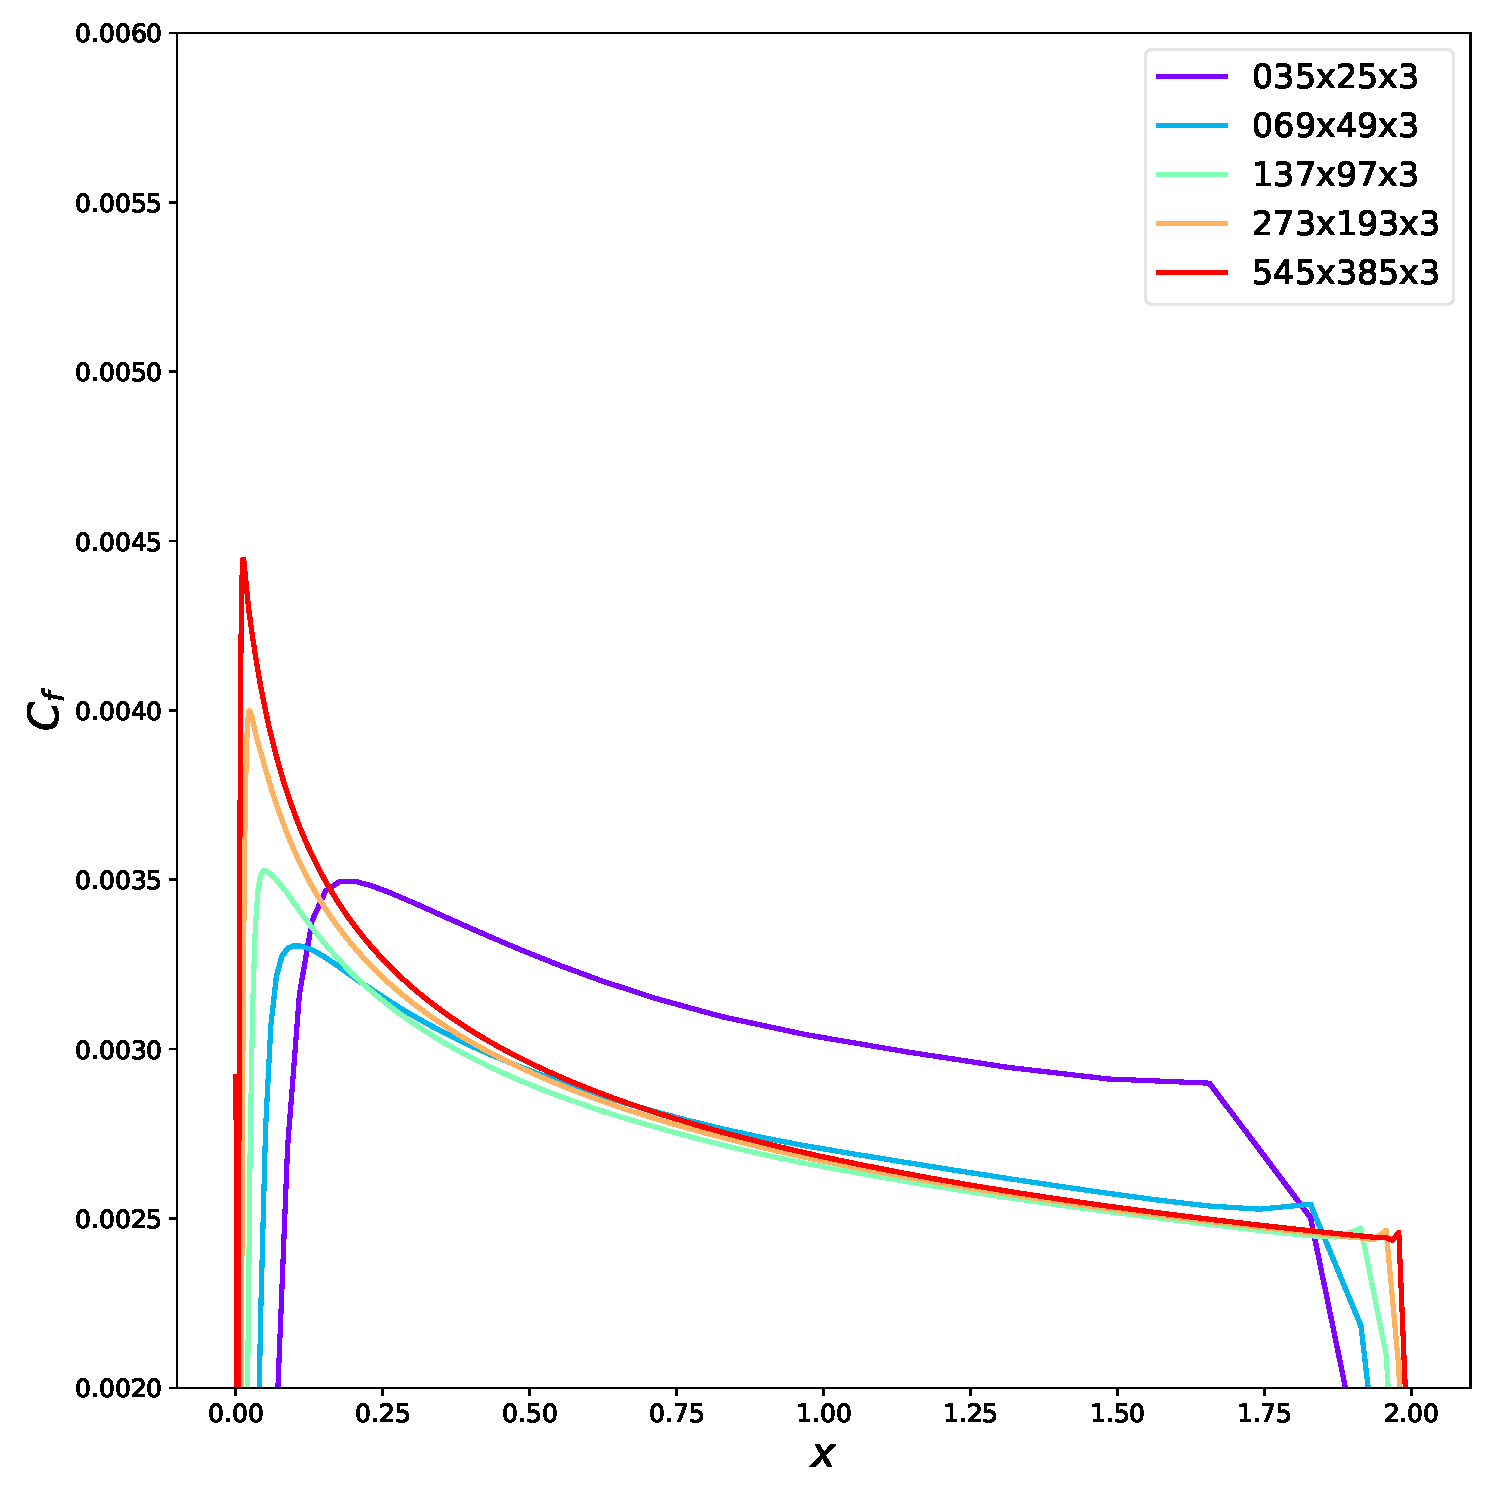
\includegraphics[width=0.7\textwidth]{figs/flat/skin_friction_grid.pdf}
  \caption{Flat Plate (Syn3D): Coefficient of skin friction on various grids.}
  \label{fig:synflatcfstudy}
\end{figure}

\begin{figure}[ht!]
\centering
\begin{subfigure}{.45\textwidth}
  \centering
  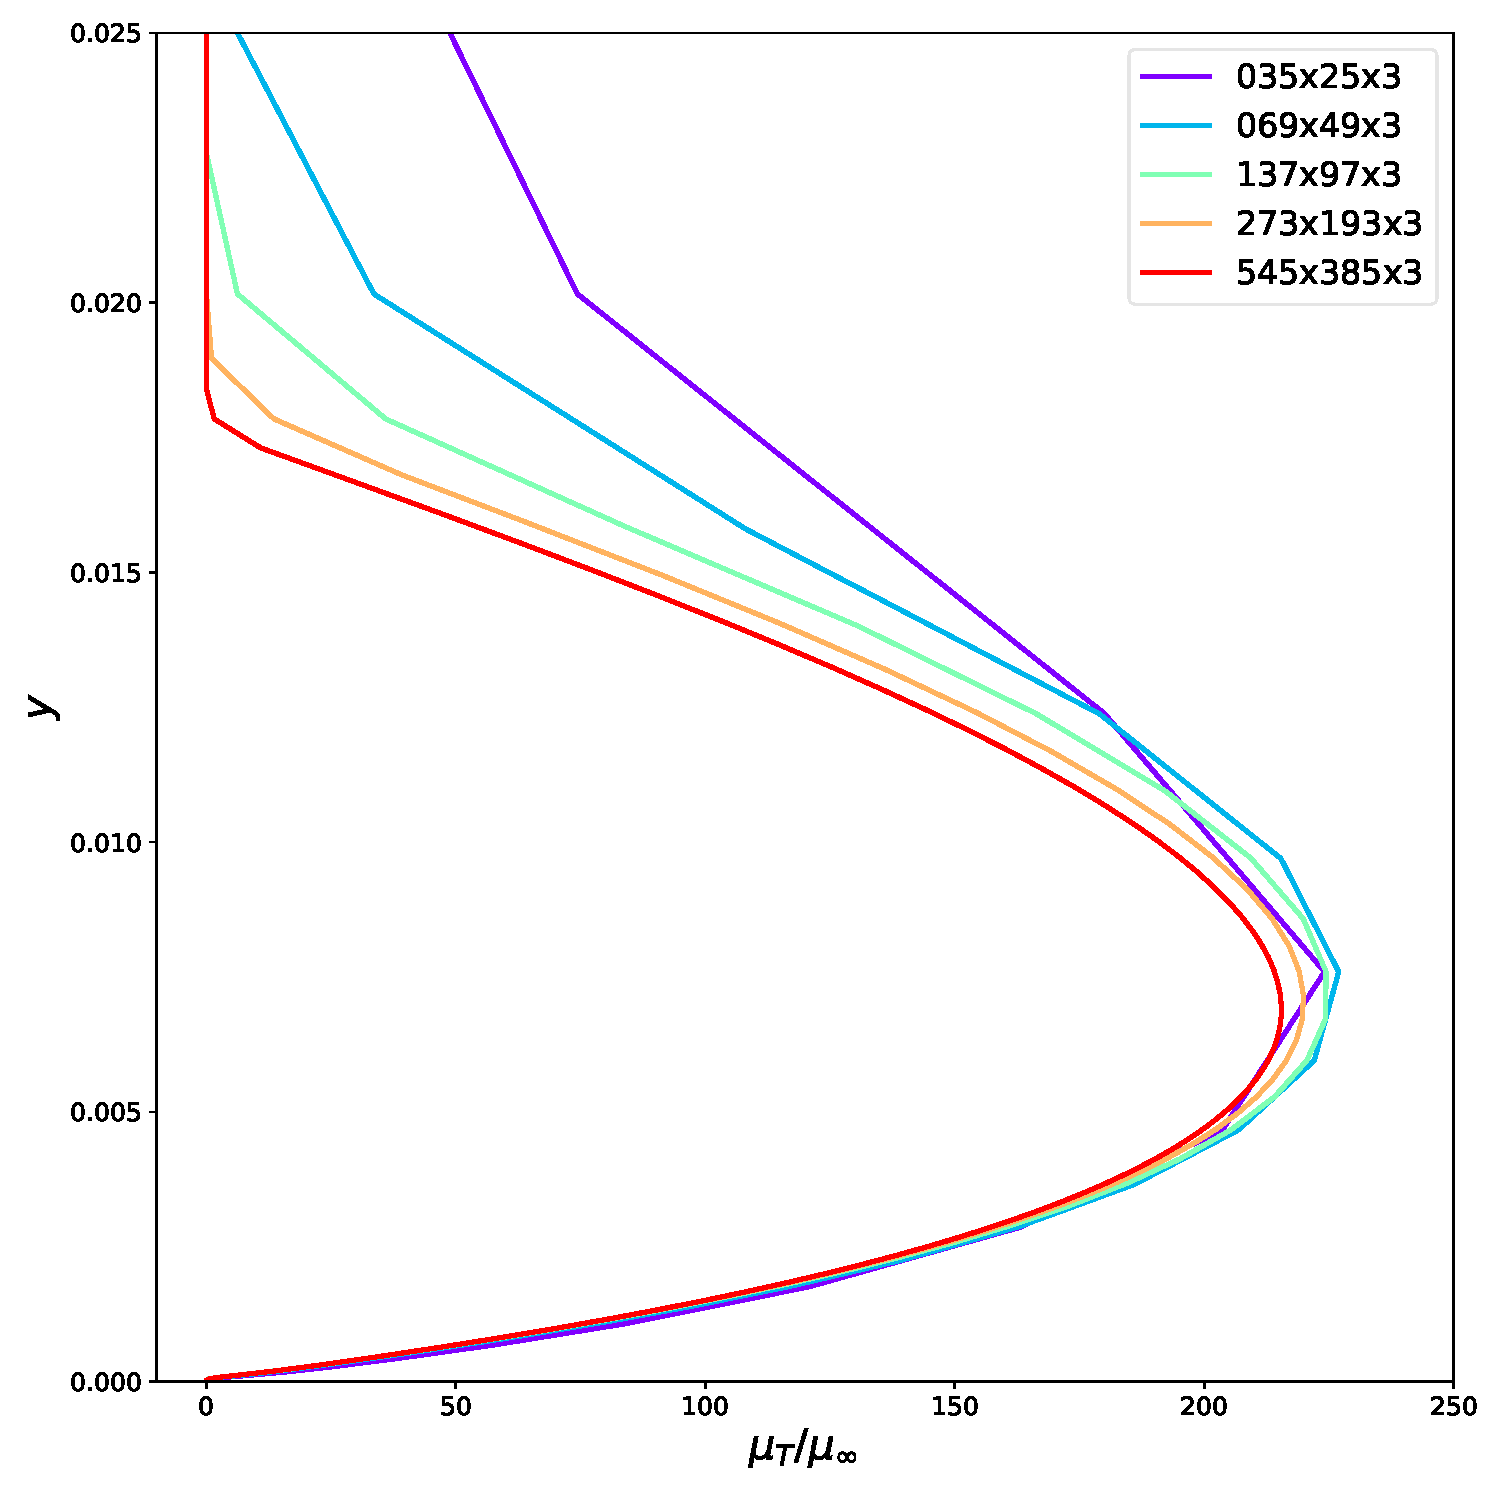
\includegraphics[width=1.0\textwidth]{figs/flat/rev_grid.pdf}
  \caption{Dimensionless eddy viscosity}
\end{subfigure}%
\begin{subfigure}{.45\textwidth}
  \centering
  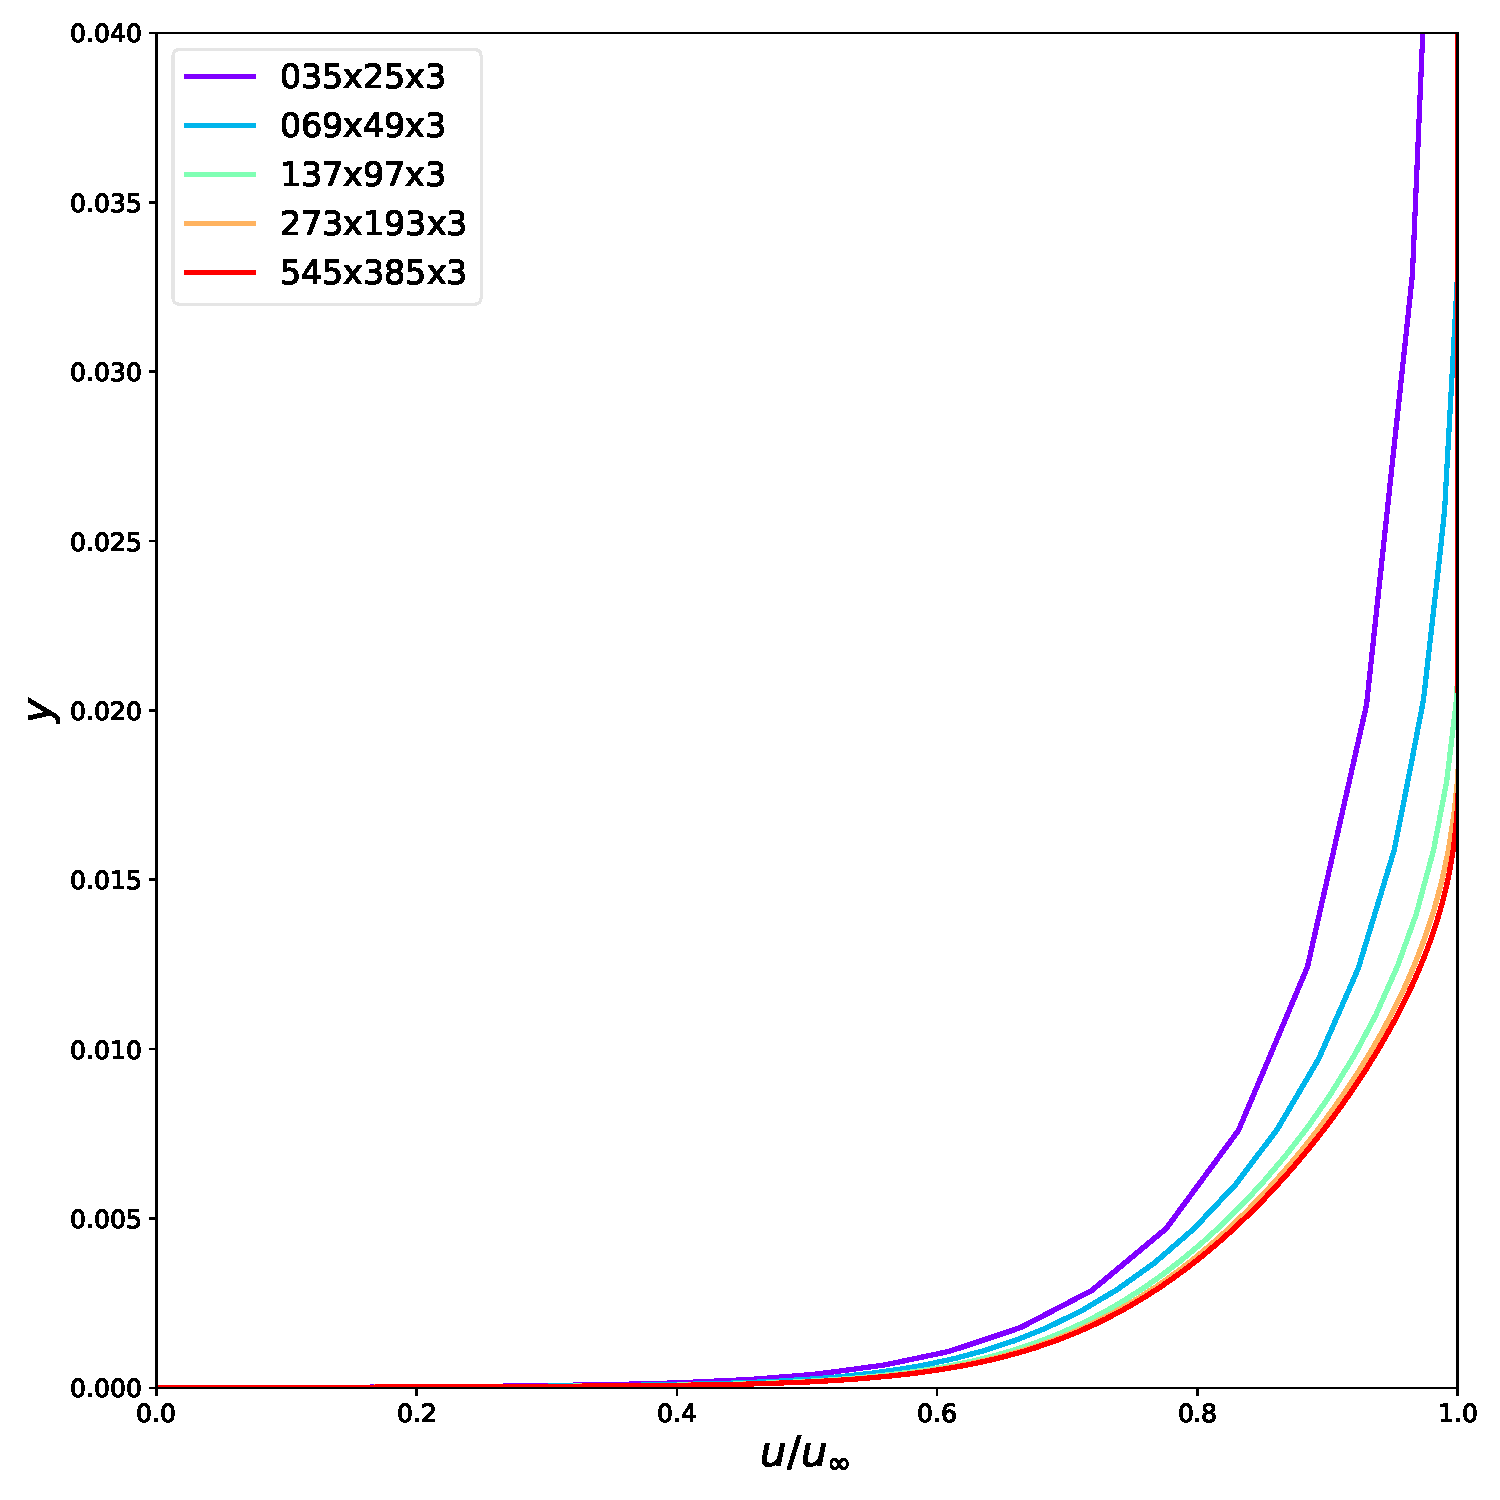
\includegraphics[width=1.0\textwidth]{figs/flat/u097_grid.pdf}
  \caption{Dimensionless velocity}
\end{subfigure}
\caption{Flat Plate (Syn3D): Profiles at $x=0.97$ for various grid sizes.}
\label{fig:synflatprofilestudy}
\end{figure}
